\documentclass{mini}

% PACKAGES
%------------------------------------------------------------------------------%
\usepackage[utf8]{inputenc}
\usepackage{tikz}
\usepackage{pgfplots}
\usepackage{wrapfig}

\usepackage{amsmath}

\DeclareMathOperator*{\argmin}{arg\,min} %argmin

\usepackage{floatrow}
% Table float box with bottom caption, box width adjusted to content
\newfloatcommand{capbtabbox}{table}[][\FBwidth]
\usepackage{caption}
\usepackage{subcaption}
\captionsetup{compatibility=false}

%%%

\usepackage{array}
% For tabulars
\newcolumntype{P}[1]{>{\centering\arraybackslash}p{#1}}


\usepackage{pdfpages}
\usepackage{graphicx}
\usepackage{longtable}
%\usepackage[export]{adjustbox}
%\usepackage{tabu}
\usepackage{xcolor,colortbl}
\usepackage{caption}
\usepackage{subcaption}
\usepackage{float}
\usepackage{wrapfig}
\usepackage{amsfonts}

%-------------------------------------------
% Group Plots
%-------------------------------------------
\usepackage{xcolor} % Colors

\usepackage{tikz}
\usepackage{keyval}
\usepackage{pgfplots} % Bar charts

\usepgfplotslibrary{groupplots}

%\usepackage{groupplots}
%\usepgfplotslibrary{groupplots}
\pgfplotsset{compat=newest}


%
% Define bar chart colors
%
\definecolor{bblue}{HTML}{4F81BD}
\definecolor{rred}{HTML}{C0504D}
\definecolor{ggreen}{HTML}{9BBB59}
\definecolor{ppurple}{HTML}{9F4C7C}


%%%%%%%%%%%%%%%%%%%%%%%%%%%%%%%%%%%%%%%%%
%           START OF COMMANDS
%%%%%%%%%%%%%%%%%%%%%%%%%%%%%%%%%%%%%%%%%


%%%%%%%%%%%%%%%%%%%%%%%%%%%%%%%%%
% Save results to be later used in addBarPlotResults
% #1: Train Small
% #2: Train Big
% #3: Train All
% #4: Test
%%%%%%%%%%%%%%%%%%%%%%%%%%%%%%%%%
\newcommand{\saveResultsFirst}[4]{
    \def\TrainSmallFirst{#1}%
    \def\TrainBigFirst{#2}%
    \def\TrainAllFirst{#3}%
    \def\TestFirst{#4}%
}

%%%%%%%%%%%%%%%%%%%%%%%%%%%%%%%%%
% Save results to be later used in addBarPlotResults
% #1: Train Small
% #2: Train Big
% #3: Train All
% #4: Test
%%%%%%%%%%%%%%%%%%%%%%%%%%%%%%%%%
\newcommand{\saveResultsSecond}[4]{
    \def\TrainSmallSecond{#1}%
    \def\TrainBigSecond{#2}%
    \def\TrainAllSecond{#3}%
    \def\TestSecond{#4}%
}

%%%%%%%%%%%%%%%%%%%%%%%%%%%%%%%%%
% Adds Results to Bars labeled by #1, #2
%
% Label #1 is used for saveResultsFirst
% Label #2 is used for saveResultsSecond
%
%%%%%%%%%%%%%%%%%%%%%%%%%%%%%%%%%
\newcommand{\addBarPlotResults}[2]{
    % TRAINING |w| < C    
    \addplot[style={bblue, fill=bblue, mark=none}]
    coordinates 
    {
        (#1,  \TrainSmallFirst)
        (#2,  \TrainSmallSecond)
    };
    
    % TRAINING |w| > C
    \addplot[style={rred, fill=rred, mark=none}]
    coordinates 
    {
        (#1,  \TrainBigFirst)
        (#2,  \TrainBigSecond)
    };
    
    % TRAINING ALL
    \addplot[style={ggreen, fill=ggreen, mark=none}]
    coordinates 
    {
        (#1,  \TrainAllFirst)
        (#2,  \TrainAllSecond)
    };
    
    % TESTING
    \addplot[style={ppurple, fill=ppurple, mark=none}]
    coordinates 
    {
        (#1,  \TestFirst)
        (#2,  \TestSecond)
    };
}



%%%%%%%%%%%%%%%%%%%%%%%%%%%%%%%%%
% Adds needed style to pgfplot
%%%%%%%%%%%%%%%%%%%%%%%%%%%%%%%%%
\newcommand{\setPlotStyle}[0]{
    \pgfplotsset{xticklabel style={text width=2em, align=center}}
}

%%%%%%%%%%%%%%%%%%%%%%%%%%%%%%%%%
% Starts groupplot with given style
%%%%%%%%%%%%%%%%%%%%%%%%%%%%%%%%%
\newcommand{\beginGroupPlot}[0]{
    \begin{groupplot}[
        group style={group size= 2 by 2,  vertical sep=50pt},
        height = 5.5cm, 
        ybar=4*\pgflinewidth, 
        ymin=0, 
        ymax=1,
        width  = 0.37*\textwidth, 
        enlarge x limits={abs=0.85cm}, 
        major x tick style = transparent, 
        ymajorgrids = true, 
        symbolic x coords={
            C=4,
            C=4 Q=3,
            C=4 Q=4,
            C=4 Q=5,
            C=4 Q=6,
            C=4 Q=7,
            C=4 Q=8,
            C=4 Q=9,
            C=4 Q=10,
            C=4 Q=11,
            C=4 Q=12,
            C=4 Q=13,
            C=4 Q=14,
            C=4 Q=15,
            C=5,
            C=5 Q=3,
            C=5 Q=4,
            C=5 Q=5,
            C=5 Q=6,
            C=5 Q=7,
            C=5 Q=8,
            C=5 Q=9,
            C=5 Q=10,
            C=5 Q=11,
            C=5 Q=12,
            C=5 Q=13,
            C=5 Q=14,
            C=5 Q=15
        },
        xtick = data, 
        scaled y ticks = false, 
        legend cell align=center, 
        legend columns=1,
        legend style={
            at={(1.45, 0.45)}, 
            anchor=north,
        }
        ]
    }%beginGroupPlot
    
    %%%%%%%%%%%%%%%%%%%%%%%%%%%%%%%%%
    % Sets legends for Bar plot
    %%%%%%%%%%%%%%%%%%%%%%%%%%%%%%%%%
    \newcommand{\setPlotLegend}[0]{
        \legend{Training $|w|<C$,  Training $|w|>C$,  Training All,  Testing}
    }
    
%%%%%%%%%%%%%%%%%%%%%%%%%%%%%%%%%%%%%%%%%
%           END OF COMMANDS
%%%%%%%%%%%%%%%%%%%%%%%%%%%%%%%%%%%%%%%%%



% COMMANDS
%------------------------------------------------------------------------------%

%%%%%%%%%%
% FUNCTION:
% classificationLanguage
%%%%%%%%%%%
\newcommand{\classificationLanguage}{
    L_{C}
}

%%%%%%%%%%
% FUNCTION:
% transformationPrecision
% ARGS:
% #1 - The alphabet
% #2 - The arguments of the transformation precision function
%%%%%%%%%%%
\newcommand{\transformationPrecision}[2]{
    P_{T_{#1}}(#2)
}

\newcommand{\umlPath}[1]{
    ../uml/#1
}

%%%%%%%%%%
% FUNCTION:
% featureTransformationSymbol
% ARGS:
% #1 = The alphabet
% OUTPUT:
% Syntax of the feature transformation of a single symbol
%%%%%%%%%%%
\newcommand{\featureTransformationSymbol}[1]{
    \rightarrow^{#1}
}

%%%%%%%%%%
% FUNCTION:
% featureTransformationWord
% ARGS:
% #1 = The alphabet
% OUTPUT:
% Syntax of the feature transformation of a word
%%%%%%%%%%%
\newcommand{\featureTransformationWord}[1]{
    \rightarrow^{#1^{*}}
}

%%%%%%%%%%
% FUNCTION:
% featureTransformationLanguage
% ARGS:
% #1 = The alphabet
% OUTPUT:
% Syntax of the feature transformation of a language
%%%%%%%%%%%
\newcommand{\featureTransformationLanguage}[1]{
    \rightarrow^{#1^{**}}
}

%%%%%%%%%%
% FUNCTION:
% featureNorm.
% ARGS:
% #1 = The feature vector
% OUTPUT:
% Syntax of feature vector normalization
% NOTE:
% Must be surranded by dollars: $\featureNorm{f}$
% Unless of course it is used in an equation
%%%%%%%%%%%
\newcommand{\featureNorm}[1]{
    ||#1||
}

% TITLE
%------------------------------------------------------------------------------%
\title{Finite automata for pattern recognition}
\titleaux{Automaty skończone w problemie rozpoznawania wzorców}
\author{Jakub Ciecierski, Bartlomiej Dybisz}
\supervisor{prof. nzw. dr hab. inż. Wladyslaw Homenda}
\type{bachelor}
\discipline{Computer Science}
\monthyear{december 2015}
\date{\today}
\album{123456}

%------------------------------------------------------------------------------%

\begin{document}
\maketitle
\tableofcontents

\chapter*{Introduction}
%---------------------------------------------------------------
Recognizing faces, discriminating between apple and oranges or understand spoken words are tasks, which are remarkably easy to processes for most of us, but happens to be astoundingly complex processes for machines. Although lately, we develop vast amount of techniques and algorithms to cope with pattern searching problem, it was implicitly used over centuries. For instance, the extensive astronomical observations of Tycho Brahe in the 16th century allowed Johannes Kepler to discover the empirical laws of
planetary motion, which in turn provided a springboard for the development of classical mechanics \cite{bishop_book}.

Automatic pattern recognition is usually considered as an engineering area which focusses on the development and evaluation of systems that imitate or assist humans in their ability of recognizing patterns \cite{duch_uuu}. Normally system, which recognizes patterns, consists of many intermediate elements, among which one can find a classifier. Following paper introduce a novel approach for building classifier based on  Deterministic Finite Automaton (further referred as DFA). Such an automaton will be able to distinguish between input objects and classify them correctly. The paper copes only with problem of classifier construction, hence it may be useful for various input data types like e.g. hand written letters or gesture patterns. 

Authors provide step-by-step explanation of each part along with mathematical background needed to understand theory behind the project.

To start with, in chapter~\ref{ch:prelim} preliminary mathematical knowledge is presented. In chapter~\ref{ch:lan_theory} we explain the first step of classifier construction which is the the process of word generation.

Finally the architecture side of the project is introduced in chapter~\ref{ch:domain}.

\chapter{Preliminaries}\label{chap:prelim}
%---------------------------------------------------------------------
Following chapter provides summary of mathematical background needed to proceed with the paper. We assume that reader is familiar with basic concepts of language theory such as: what is a language and what does it mean that it is regular. In addition, it is crucial for reader to understand the idea of equivalence classes, because they comprise a very essence and motivation of this work. Finally, we are trying to (as quickly as possible) dive into theorems and definitions which are useful from the point of view of further application, rather than spending time on deriving knowledge from beginning.
%---------------------------------------------------------------------
%---------------------------------------------------------------------
\section{Myhill-Nerode}
\begin{definition} \label{def:myhill}
    Relation induced by language $L$ is a binary relation $R_{L}$ in the set of words over alphabet of $L$ such that:
    \[
    (\forall{u,v \in \Sigma^{*}})(u R_{L} v \equiv ((\forall z \in \Sigma^{*}) uz \in L \Leftrightarrow vz \in L))
    \]
\end{definition}
What is more, we know that $R_{L}$ is an equivalence relation, hence it divides $\Sigma^{*}$ into equivalence classes.

In the theory of formal languages, the $Myhill-Nerode$ theorem provides a necessary and sufficient condition for a language to be regular. The theorem is named for John Myhill and Anil Nerode, who proved it at the University of Chicago in 1958 (Nerode 1958) \cite{Myhill_Nerode}.

\begin{theorem}[Myhill-Nerode Theorem]\label{Theorem:Myhill_Nerode}
    The following conditions are equivalent:
    \begin{enumerate}
        \item a language $L$ is accepted by a deterministic finite automaton $M = (Q,\Sigma,\delta,q_0,F)$,
        \item a language $L$ is a union of some classes of a right invariant equivalence relation with finite index,
        \item the relation $R_{L}$ induced by a language $L$ has finite index.
    \end{enumerate}
\end{theorem}

%---------------------------------------------------------------------
%---------------------------------------------------------------------
\section{Hamming Distance} \label{sec:hamming}

\begin{definition}
Hamming distance $H_d$ between two string of the same length is the number of positions at which the corresponding symbols differ.
\end{definition}

\begin{example} 
Let $w = John$ and $v = Jhon$. Notice that the symbols at positions two and three differ. Thus the Hamming distance between these two strings is $H_d(w,v) = 2$.
\end{example}

%---------------------------------------------------------------------
%--------------------------------------------------------------------
\section{Cluster Evaluation} \label{sec::cluster}

Clustering is a method of segregating elements of a given data set into groups. Elements similar to each other should fall into one group while dissimilar elements are supposed to be separated.

The problem arises when no prior information about the structure of the data is given. At that point we can not simply assume number of clusters for the partitioning. The methods that estimate the optimal number of clusters in the given data set are now presented.

%---------------------------------------------------------------------
%---------------------------------------------------------------------
%---------------------------------------------------------------------
\subsection{K-Means}

K-means algorithm is a tool for clustering a given data set.
The goal of that algorithm is to partition a data set $X$ of size $n$ into $k$ clusters, where each $x_{j}\in X$ is assigned a single cluster. In order to do that, we find cluster centroids $\mu_{i}, i=1,\ldots,k$ that minimize the distance from the elements from data set. Formally k-means solves the following optimization problem:
\begin{equation}
    \argmin_{C}\sum_{i=1}^{k}\sum_{x\in C_{i}} d(x,\mu_{i})
\end{equation}
where $C_{i}$ is the set of elements that correspond to $i$-th cluster and $d(x,\mu_{i})$ is a~chosen distance measure between element $x$ and the cluster center $\mu_{i}$. At the first stage of the algorithm k centroids $\mu_{i}$ are selected. Then each element is assigned to the closest cluster. The centroids are updated with the mean of all points belonging to the corresponding cluster
\begin{equation}
    \mu_{i} = \frac{1}{|C_{i}|} \sum_{x\in C_{i}} x
\end{equation}

This process is repeated until convergence. It is worth mentioning that k-means might not find the best possible 
configuration.

The following summarises the k-means algorithm:

\begin{center}
    
    
    \begin{enumerate}
        \item 
        Select $k$ initial centroids
        \item \label{enum:km_grp} 
        Group points to their closest centroids.
        \item \label{enum:km_centroids} 
        Update centroids by computing center of gravity - mean
        \item 
        Repeat~\ref{enum:km_grp} and~\ref{enum:km_centroids} until convergence or after maximum iterations.
    \end{enumerate}
    
\end{center}

The method of choosing initial centroids can have a big impact on the result and the complexity. The naive method of initialization would involve using uniform distribution to randomly select k centroids among the data set. Such approach can easily define two centroids within a single potential cluster and thus k-means can get stuck in local optimum.
The k-means++ (k-means plus plus), algorithm proposes a better solution for initialization by spreading out the centroids. At the beginning, the first centroid is chosen as usual uniformly from the data set. Then for each data point $x$ we compute $D(x)$ which defines the distance between $x$ and the nearest centroid that have already been chosen. The next centroids is chosen by selecting a point from data set using weighted probability distribution proportional to $D(x)^2$. The process is repeated until all $k$ centroids are found.

The formal flow of the algorithm is now presented:

\begin{enumerate}
    \item 
    Choose the first centroid uniformly from data set.
    \item \label{enum:kmpp_dx}
    For $x$ in data set:
    \begin{enumerate}
        \item
        Compute $D(x)$, the distance between x and its nearest centroid.
    \end{enumerate}
    
    \item \label{enum:kmpp_weight}
    Select next centroid from data set with probability:
    $\frac{D(x)^2}{\sum_{x}D(x)^2}$
    \item 
    Repeat steps~\ref{enum:kmpp_dx} and~\ref{enum:kmpp_weight} until $k$ centroids are found.
\end{enumerate}

%---------------------------------------------------------------------
%---------------------------------------------------------------------
%---------------------------------------------------------------------
\subsection{McClain-Rao}
The McClain-Rao algorithm tries to select the optimal number of clusters for given data set. Let's define few measures needed to compute McClain-Rao index. Firstly we define the sum within-cluster distances $S_w$. It sums up all the distances of any two points from the same cluster. Formally $S_w$ is defined by the equation: 
\begin{equation}
    S_w = \sum_{l=0}^{k} \sum_{i < j \in I_l} d(x_i, x_j)
\end{equation}
where $I_l$ is the set of indices of the $l$-th cluster. Let $N_w$ be the total number of distances between pairs of points belonging to the same cluster.

Further, the sum of between-cluster distances $S_b$ is the sum of distances of points belonging to different clusters. The following equations describes it:
\begin{equation}
    S_b = \sum_{l < l^{'}}^{k} \sum_{i \in I_{l}, j \in I_{l^{'}}}  d(x_i, x_j)
\end{equation}
Similarly, let $N_b$ be the total number of distances between pairs of points which do not belong to the same cluster.

Finally, The McClain-Rao index $C$ is defined by equation: 
\begin{equation}
    C =  (\frac{S_w}{N_w}) / (\frac{S_b}{N_b})
\end{equation}

$C$ is the quotient between the mean within-cluster and between-cluster distances.
Note that the smaller the value of $C$ the better the clustering.

%---------------------------------------------------------------------
%---------------------------------------------------------------------
\section{Automaton} \label{sec:autom}
%\begin{definition}
Automaton is a system of five fields:
\begin{center}
    $A = (Q, \Sigma, \delta, q_0, F)$
\end{center}

where \\
$Q$ - finite set of states. \\
$\Sigma$ - Finite input alphabet. \\
$\delta$ - transition function. $\delta: Q \times \Sigma \rightarrow Q$ \\
$q_0$ - the initial state. $q_0 \in Q$ \\
$F$ - Set of accepting states. $F \subseteq Q$ \\
%\end{definition}

Table~\ref{fig:ttable_std} shows an exmaple transition table for the standard transition $\delta: Q \times \Sigma \rightarrow Q$.

%%%
%
% Standard Transition function
%
%%%
\begin{figure}[H]
    \CenterFloatBoxes
    \begin{floatrow}
        
        \ttabbox
        {
            \centering
            \setlength{\tabcolsep}{15pt}
            \renewcommand{\arraystretch}{1.5}
            \begin{tabular}{|P{1.0cm} || P{0.6cm} | P{0.6cm} |}
                \hline
                $\delta$ & a & b \\
                \hline
                \hline
                $\rightarrow q^-$ 		& $q_0$ & $q_1$ \\
                \hline
                $q_0 \rightarrow$ 		& $q_R$ & $q_R$ \\
                \hline
                $q_1 \rightarrow$ 		& $q_1$ & $q_1$ \\
                \hline
                $q_R$  					& $q_R$ & $q_R$ \\
                \hline
            \end{tabular}
        }
        {\caption{Transition table for A with $\delta: Q \times \Sigma \rightarrow Q$}\label{fig:ttable_std}}
        
        %\ffigbox
        %  {\includegraphics[width=0.35\textwidth]%{images/automaton_example.jpg}}
        %  {\caption{Example of Automaton %A}\label{fig:automaton_ex}}
        %\killfloatstyle
        
    \end{floatrow}
\end{figure}


The binary representation of automaton might perhaps provide more adequate solution for a computer. Thus a new transition function is defined, $\delta^{'}: Q \times \Sigma \times Q \rightarrow \{0,1\}$. It simply provides an answer whether there exists a transition between two states for a given symbol. For example, by looking at figure~\ref{fig:ttable_std} we can define value for $\delta^{'}(q^-,a,q^0) = 1$, since there exists a transition from $q^-$ to $q^0$ through symbol $a$. The entire automaton is presented in figure~\ref{fig:ttable_bin}.


%%%
%
% Binary transition function.
%
%%%
\begin{figure}[H]
    \begin{center}
        
        \setlength{\tabcolsep}{4pt}
        \renewcommand{\arraystretch}{1.4}
        
        \begin{subfigure}{.5\textwidth}
            
            \centering
            \begin{tabular}{|P{1.0cm} || P{0.8cm} | P{0.8cm} | P{0.8cm} | P{0.8cm}|}
                
                \hline
                a & $\rightarrow q^-$ & $q_0 \rightarrow$ & $q_1 \rightarrow$ & $q_R$ \\
                \hline
                \hline
                $\rightarrow q^-$ 		& $0$ & $1$ & $0$ & $0$ \\
                \hline
                $q_0 \rightarrow$ 		& $0$ & $0$ & $0$ & $1$ \\
                \hline
                $q_1 \rightarrow$ 		& $0$ & $0$ & $1$ & $0$ \\
                \hline
                $q_R$  					& $0$ & $0$ & $0$ & $1$ \\
                \hline
                
            \end{tabular}
            
            \caption{Transition table for symbol $a$}
            \label{fig:ttable_bin_a}	
            
        \end{subfigure}%
        \begin{subfigure}{.5\textwidth}
            
            \centering
            \begin{tabular}{|P{1.0cm} || P{0.8cm} | P{0.8cm} | P{0.8cm} | P{0.8cm}|}
                
                \hline
                b & $\rightarrow q^-$ & $q_0 \rightarrow$ & $q_1 \rightarrow$ & $q_R$ \\
                \hline
                \hline
                $\rightarrow q^-$ 		& $0$ & $0$ & $1$ & $0$ \\
                \hline
                $q_0 \rightarrow$ 		& $0$ & $0$ & $0$ & $1$ \\
                \hline
                $q_1 \rightarrow$ 		& $0$ & $0$ & $1$ & $0$ \\
                \hline
                $q_R$  					& $0$ & $0$ & $0$ & $1$ \\
                \hline
                
            \end{tabular}
            
            \caption{Transition table for symbol $b$}
            \label{fig:ttable_bin_b}
            
        \end{subfigure}%
        
        
        \caption{Transition tables for symbols $a$ and $b$, making up the entire transition function $\delta^{'}: Q \times \Sigma \times Q \rightarrow \{0,1\}$}
        
        \label{fig:ttable_bin}
    \end{center}
\end{figure}

It is important to note that to preserve determinism, there must exist exactly one transition from any state for a given symbol. In other words in each transition table for $\delta^{'}$ a single row must be a sequence of $0s$ and a single digit $1$.

%---------------------------------------------------------------------
%---------------------------------------------------------------------
%---------------------------------------------------------------------
\subsection{Decoding} \label{sec:auto_dec}

Let us denote the number of states by $n = |Q|$, and number of symbols in alphabet by $r = |\Sigma|$. Further, we shall enumerate all states 	$Q = \{q_1, q_2, \ldots, q_n\}$, and all the symbols in the alphabet 	$\Sigma = \{x_1, x_2, \ldots, x_r\}$. We will also define the size of automaton $s(A) = n*r$.

We now turn to the binary approach of transition function $\delta^{'}$ described in the figure~\ref{fig:ttable_bin}. Notice that each table for symbol $x_l$ for $l = 1,2, \dots, r$ has exactly $n$ rows. Furthermore, we can easily decode each $row_{x_l, i}$ into a natural number. Let $j$ be the index of occurrence of digit $1$ in the $row_{x_l, i}$. The natural number $j$ will then be a decoding of $row_{x_l, i}$. Decoding of a single table will be a vector of $n$ natural numbers. Notice that the first element of such vector will correspond to the transition of initial state. Now the last objective of representing the automaton is to combine all vectors, each corresponding to transition table for symbol $x_{l}$. We simply append all vectors in order of the symbols' enumeration. The entire proceeder is illustrated in figure~\ref{fig:encoding}. Firstly, in figures~\ref{fig:encoding_a} and~\ref{fig:encoding_b} we see decoding of transition tables for symbols $a$ and $b$ respectively. Finally the figure~\ref{fig:encoding_both} shows entire decoding of automaton $A$. We will call such decoding a direct or natural decoding of automaton with binary transition function.

%%%
%
% Natural encoding
%
%%%
\begin{figure}[H]
    \begin{center}
        
        \setlength{\tabcolsep}{1pt}
        \renewcommand{\arraystretch}{1.9}
        
        \begin{subfigure}{.5\textwidth}
            \centering
            
            \begin{tabular}{|P{.9cm} | P{0.9cm} | P{0.9cm} | P{0.9cm} | P{0.9cm} |}
                \hline
                $r_{a,1}$  & $r_{a,2}$ & $r_{a,3}$ & $r_{a,4}$ \\
                \hline
                \hline
                $2$  & $4$ & $3$ & $4$ \\
                \hline	
            \end{tabular}
            \caption{Natural decoding of Transition table \\presented in figure~\ref{fig:ttable_bin_a}}
            \label{fig:encoding_a}
        \end{subfigure}%
        \begin{subfigure}{.5\textwidth}
            \centering
            
            \begin{tabular}{|P{.9cm} | P{0.9cm} | P{0.9cm} | P{0.9cm} | P{0.9cm} |}
                \hline
                $r_{b,1}$  & $r_{b,2}$ & $r_{b,3}$ & $r_{b,4}$ \\
                \hline
                \hline
                $3$  & $4$ & $3$ & $4$ \\
                \hline	
            \end{tabular}
            \caption{Natural decoding of Transition table \\presented in figure~\ref{fig:ttable_bin_b}}
            \label{fig:encoding_b}
        \end{subfigure}
        
        \begin{subfigure}{.5\textwidth}
            \centering
            
            \begin{tabular}{|P{.9cm} | P{0.9cm} | P{0.9cm} | P{0.9cm} | P{0.9cm} |P{.9cm} | P{0.9cm} | P{0.9cm} | P{0.9cm} | P{0.9cm} |}
                \hline
                $r_{a,1}$  & $r_{a,2}$ & $r_{a,3}$ & $r_{a,4}$ & $r_{b,1}$  & $r_{b,2}$ & $r_{b,3}$ & $r_{b,4}$ \\
                \hline
                \hline
                $2$  & $4$ & $3$ & $4$ & $3$  & $4$ & $3$ & $4$ \\
                \hline	
            \end{tabular}
            \caption{Natural decoding of all Transition tables presented in figure~\ref{fig:ttable_bin}. The abbreviation $r_{x,i}$, represents the $i$-th row of table corresponding to symbol x}
            \label{fig:encoding_both}
        \end{subfigure}
        
        \caption{Natural decoding of Automaton A}
        \label{fig:encoding}
    \end{center}
\end{figure}

Natural decoding of an automaton with $n$ states and $r$ symbols in the alphabet will be a vector of size $n*r$. First element of each sub vector will indicate the transition for initial symbol. The retrieval of elements corresponding to transitions of specific symbols is omitted due to its triviality.

Formally, each element of the decoding vector is a natural number greater than 0. Summarizing, the elements of each dimension, take values from the discrete set $\{1,2, \ldots, n\}$.

It is worth mentioning, that in such decoding the information about accepting states is lost.


%---------------------------------------------------------------
\chapter{Pattern Recognition} \label{chap:patt_rec}

Chapter provides brief introduction to pattern recognition discipline . Via various examples, it tries to supply reader with general intuition about subject. 


\subsection{Basics}

The field of pattern recognition is concerned with the automatic discovery of regularities in data through the use of computer algorithms and with the use of these regularities to take actions such as classifying the data into different categories \cite{bishop_book}.

Best example to start with, are hand written digits. Let us consider figure \ref{fig:handwritten_ex}. It presents set of digits created by user manually. Images are binary i.e. pixel saturation is either none (black color) or maximal (white ones) - no other values are present. Each digit is bounded in $20 \times 20$ box, hence it occupies 400 pixels. 

Those pixels can be though of as a vector of length 400, where entries are values of consecutive pixels. The goal is to create algorithm, which takes such a vector and produce output telling, what number has been provided. In our example, such a program would accept vector of 400 pixels and output one of the following values: 0, 1, 2, 3, 4, 5, 6, 7, 8 or 9. Since there are vast amount of writing styles and more or less each one of us uses pen in a different way, approach to the problem is not straight forward. 

\begin{wrapfigure}{r}{0.5\textwidth}
  \begin{center}
    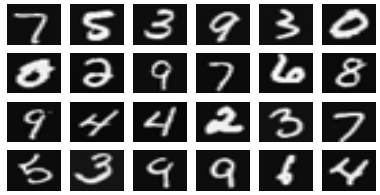
\includegraphics[width=0.7\textwidth]{images/handwritten_digits_example.png}
  \end{center}
  \caption{Example of $20 \times 20$ handwritten digits.}
  \label{fig:handwritten_ex}
\end{wrapfigure}

One of the most effective solutions would be to provide our algorithm with large amount of such digits images to tune parameters of adaptive model. Such a set of images is called training set and the stage is known as a training phase. In it also a common practice to preprocess images to reduce dimensionality. For example if we would assume that our algorithm must run in real-time, processing large amount of pixels would be computationally inefficient. One of the mostly used technique assumes that one should consider only some of the images features. Features should be quick to compute and represent information that varies between images, hence can be used to discriminate between them. It is worth stressing out that preprocessing stage is crucial for overall system accuracy.


\subsection{Types of Learning}
One can distinguish between 3 main approaches to the learning procedure: supervised, unsupervised and semi-supervised. Following paragraphs will discuss them briefly - just to grab the idea.

\begin{wrapfigure}{l}{0.4\textwidth}
  \begin{center}
    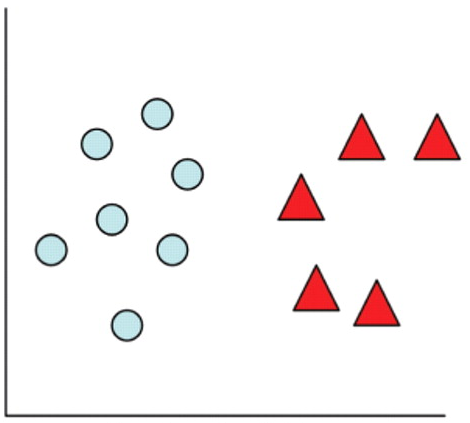
\includegraphics[width=0.55\textwidth]{images/supervised_graph.png}
  \end{center}
  \caption{Labeled data}
  \label{fig:handwritten_ex}
\end{wrapfigure}


\textbf{Supervised Learning} basically corresponds to processing data with a priori knowledge about its types. As in example from previous section, one is in possession of knowledge about types of digits. As said before algorithm must label input data as one of the following digits: 0, 1, 2, 3, 4, 5, 6, 7, 8 or 9. No other types are considered and all are known, hence the example is of supervised type. One can distinguish two approaches, based on type of input data:
\begin{itemize}
  \item Classification - assign discrete input data to discrete categories
  \item Regression - assign continuous input data to discrete categories.
\end{itemize}

\begin{wrapfigure}{l}{0.4\textwidth}
  \begin{center}
    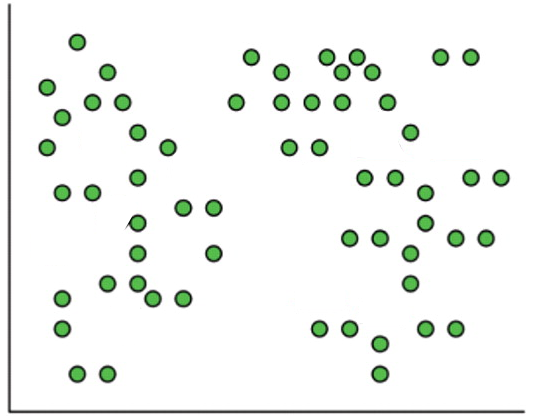
\includegraphics[width=0.55\textwidth]{images/unsupervised_graph.png}
  \end{center}
  \caption{Unlabeled data.}
  \label{fig:handwritten_ex}
\end{wrapfigure}

\textbf{Unsupervised Learning} copes with problems where there is lack of data labeling. We would for example consider our leading example as unsupervised if algorithm would be supplied only with pixel vectors with no associations to numbers they representing. The goal of unsupervised algorithm may vary from case to case, but can generally it considers following problems:

\begin{itemize}
  \item Clustering - discovering group of similar objects within data.
  \item Density Estimation - determine distribution over input space.
  \item Visualization - project from high-dimensions data to three dimensions, for the purpose of visualization
\end{itemize}

\begin{wrapfigure}{l}{0.4\textwidth}
  \begin{center}
    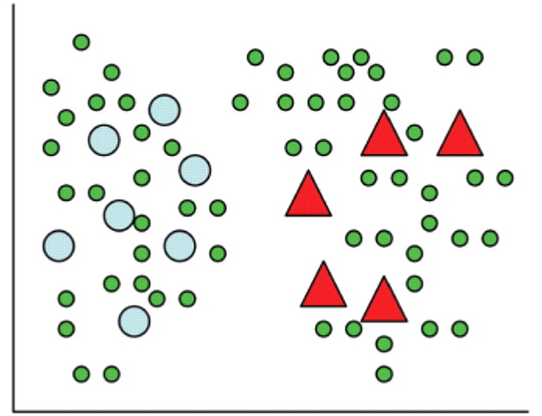
\includegraphics[width=0.55\textwidth]{images/semi_supervised_graph.png}
  \end{center}
  \caption{Labeled and unlabeled data.}
  \label{fig:handwritten_ex}
\end{wrapfigure}

\textbf{Semi-Supervised Learning} The goal of semi-supervised learning is to understand how combining labeled and unlabeled data may change the learning behavior, and design algorithms that take advantage of such a combination \cite{semi_supervised}. Often label instances are difficult, expensive, or time consuming to obtain, as they require the efforts of experienced human annotators. Because semi-it requires less human effort and gives higher accuracy, it is of great interest both in theory and in practice \cite{semi_supervised2}.


%-------------------------------------------------------------------
\pagebreak
\paragraph{}
\subsection{Quality Evaluation}\label{evaluation}
For better understanding of how quality of classification should be measured we adopt parameters and quality measures used in signal detection theory. Since these parameters are widely utilized, we do not refer to original sources here. The following parameters were used in defining several measures outlining classification's quality. These parameters create so called confusion matrix, which is given in Table~\ref{tab:conf_matrix}. The parameters given in the matrix are numbers of elements of a~testing set which have the following meaning:
\begin{itemize}
  \item $TP$ - the number of elements of the considered class correctly classified to this class,
  \item $FN$ - the number of elements of the considered class incorrectly classified to other classes,  
  \item $FP$ - the number of elements of other classes incorrectly classified to the considered class,  
  \item $TN$ - the number of elements of other classes correctly classified to other classes (no matter, if correctly, or not).  
\end{itemize}  

\begin{table}[H]
\vspace{-9pt}
\centering
\begin{tabular}{|c|c|c|}
\hline
  & & \vspace{-6pt}\\
  & \hspace{12pt}Classification to the class\hspace{12pt} & \hspace{3pt}Classification to other classes\hspace{3pt} \\
  & & \vspace{-6pt}\\
\hline 
  & & \vspace{-6pt}\\
  The class & True Positivse (TP) & False Negatives (FN) \\
  & & \vspace{-6pt}\\
\hline
  & & \vspace{-6pt}\\
  \hspace{3pt}Other classes\hspace{3pt} & False Positives (FP) &  True Negatives (TN)\vspace{3pt}\\
\hline
\end{tabular}
\vspace{9pt}
\caption{Confiusion matrix for rejecting in pattern recognition problem}
\label{tab:conf_matrix}
\end{table}

The following measures were used assess the quality of the classifier:
%\begin{flalign}
\begin{eqnarray}
  \textnormal{Accuracy}    & = &   \displaystyle\frac{\textnormal{TP+TN}}{\textnormal{TP+FN+FP+TN}}\nonumber\\
  \textnormal{Sensitivity} &\;=\;& \displaystyle\frac{\textnormal{TP}}{\textnormal{TP+FN}}\nonumber\\
  \textnormal{Precision}   & = &   \displaystyle\frac{\textnormal{TP}}{\textnormal{TP+FP}}\nonumber\\
  \textnormal{F--measure}  &\;=\;& 2\cdot\frac{\mbox{Precision}\cdot\mbox{Sensitivity}}{\mbox{Precision}+\mbox{Sensitivity}}
\end{eqnarray}

The following comments help to understand remaining of characteristics:

\begin{itemize}
  \item Accuracy is the measure of the rejecting performance. This measure describes the ability to distinguish between native and foreign elements. Of course, the higher the value of this measure, the better the identification.
  \item Precision is the ratio of the number of not rejected native elements to the number of all elements (native and foreign) not rejected. Precision evaluates the rejection ability to separate foreign elements from native ones. The higher the value of this measure, the better ability to distinguish foreign elements from native ones.
  \item Sensitivity is the ratio of the number of not rejected native elements to the number of all native ones. This measure evaluates the rejection ability to identify native elements. The higher the value of Sensitivity, the more effective identification of native elements. Unlike the Precision, this measure does not evaluate the effectiveness of separation between native and foreign elements. The higher the value of this measure, the better ability to identify native elements.
  \item Precision and Sensitivity are complementary: increasing sensitivity can cause a drop in precision since, along with increasing the number of not rejected native elements, there might be more not rejected foreign ones. It is there to express the balance between precision and sensitivity since, in practice, these two affect each other. There exists yet another characteristic that combines them: the \mbox{F--measure}. The higher the value of this measure, the better balance between identification of native elements along with separation native elements from foreign ones.
\end{itemize}
It is worth to say that other measures characterizing rejection quality can be invented, cf.~\cite{Homenda_2014}, but they are derivations from defined above.  

%---------------------------------------------------------------
\chapter{Language Theory} \label{chap:lan_theory}

The content discussed thus far, presented pattern recognition as a general problem. This chapter is considered to be a bridge between the pattern recognition world and the language and automata theory. We propose a set of procedures which help in reducing the classical problem of classification into a language theory problem. By doing so, we will be able to benefit from the prosperous theory of languages and automata.



The chapter begins with element and object transformations into words and languages, respectively.

%---------------------------------------------------------------
%---------------------------------------------------------------
\section{Transformation}\label{sec:lan_theory_transf}
This section is devoted to explaining the process of transformation of abstract objects into languages. All feature vectors are assumed to be of the same dimensions.

%---------------------------------------------------------------
%---------------------------------------------------------------
%---------------------------------------------------------------
\subsection{Word Transformation}\label{sec:lan_theory_transf_word}


Let us consider a feature vector~$f = [c_{1},c_{2},\ldots,c_{m}]$ and an alphabet $\Sigma=\{a_{1}, a_{2}, \ldots, a_{r} \}$. Notice that $|\Sigma|=r$.
The first step of transformation process will include transforming each feature into a symbol. Recall that different features may belong to different intervals. For that reason, all features need to be normalized to a common interval. Let $\featureNorm{f}$, denote a normalized feature vector. For convenience, the normalized interval will be defined by the size of the alphabet, namely $c_{i} \in \langle 0 , r \rangle$. The details of normalization are presented later in this section.

Having the interval conveniently normalized, we can now easily define the transformation of a single feature to a symbol by partitioning the intervals into $r$ sub-intervals: $x_1, x_2,\ldots,x_r$. We can now easily translate feature $c_i \in x_{j}$ by assigning the corresponding symbol $a_{j}$.

Formally the transformation of a single feature is defined by the follow equation:

\begin{equation*}
c_i \featureTransformationSymbol{\Sigma}
\begin{cases}
a_1 & \text{for } c_{i} \in  \langle 0 , 1) \\
a_2 & \text{for } c_{i} \in  \langle 1 , 2) \\
a_3 & \text{for } c_{i} \in  \langle 2 , 3) \\
&\makebox[\widthof{${}\rightarrow{}$}][c]{\vdots} \\
a_{r} & \text{for } c_{i} \in \langle r -1, |\Sigma|  \rangle
\end{cases})
\end{equation*}

Having completed the transformation of all features of a given feature vector, the next step includes concatenating all consecutive symbols to create a word defining the feature vector. Formally, we define the word transformation as: $f \featureTransformationWord{\Sigma} w$, where $w \in \Sigma^*$ 

        
\begin{example} {\bf Word Transformation}\\
    Let $\Sigma =\{a,b\}$ be the alphabet and $\featureNorm{f} = [c_{1},c_{2},c_{3}]$ be a feature vector with normalized features to interval $\langle 0,2 \rangle$.
    Let $c_{1}=0.6$, $c_{2} = 1.5$, $c_{3} = 1.9$.
    By applying the feature transformation for all features we get:
    \begin{center}
        $c_{1} \featureTransformationSymbol{\Sigma} a$,
        $c_{2} \featureTransformationSymbol{\Sigma} b$,
        $c_{3} \featureTransformationSymbol{\Sigma} b$.
    \end{center}
    Finally the concatenation of consecutive symbols yields a word defining the feature vector $\featureNorm{f} \featureTransformationWord{\Sigma} w = abb$.
\end{example}

The following section focuses on the normalization process and mathematical details of transformation.

%---------------------------------------------------------------
%---------------------------------------------------------------
%---------------------------------------------------------------
%---------------------------------------------------------------
\subsubsection{Normalization} \label{sec:lan_theory_word_transf_norm}
One of the first challenges that appears during tackling the problem is features vector coding. By coding we understand changing vectors of real numbers into words over some alphabet. In case when the application has been supplied by real data, program needs to load tables and interpret them somehow. Following subsection describes process in general using mathematical description.

First of all let us assume that file has been already loaded and we are provided with set of features vectors: 

\[ F = \{ f_1 , f_2, \cdots , f_n \} \]

, where each $f_i \in \mathbb{R}^{1 \times m}$, for $i \in \langle 1,n \rangle$.
Next we assume that set of $m$ features 

\[ C = \{ c_1 , c_2, \cdots , c_m \}\] 

has been supplied as well. With this knowledge we represent each vector from set $F$ as: 

\begin{align*}
f_1 = [ c_{11} \; c_{12} \; \cdots \; c_{1m}] \\
f_2 = [ c_{21} \; c_{22} \; \cdots \; c_{2m}] \\
\cdots \\
f_n = [ c_{n1} \; c_{n2} \; \cdots \; c_{nm}] 
\end{align*}

, where entries of each vector represents values for consecutive features $c_1, c_2 \cdots , c_m$. We will use $c_{ij }\in f_i$ notation to refer to $j$th element of feature vector $f_i$ 

Since each feature from $C$ can take values from different intervals we decided to normalize all of them. There are two functions which will be useful in this process:
\begin{align*}
max : \{c_1, c_2, \cdots, c_m\} \rightarrow \mathbb{R} \\
min : \{c_1, c_2, \cdots, c_m\} \rightarrow \mathbb{R}
\end{align*}
Given feature $c_j$ for $j \in \langle 1, m \rangle$, they specify upper and lower boundary of the interval within which $c_j$ is captured. For example if $c_3$ takes values from interval $\langle -1 , 5 \rangle$, $max(c_3) = 5$ and $min(c_3 = -1)$.

Recall that $\Sigma$ represents an alphabet. Let us assume that $\Sigma = \{a_1 , a_2, \cdots, a_{|\Sigma|}\}$. Our goal is to hold all values of features vectors in $\langle 0 , |\Sigma| \rangle$ interval. To perform such conversion we will use following operation:
\begin{equation}
IntCnv(f_i) \Leftrightarrow (\forall{c_{ij} \in f_i})(c_{ij} =  \frac{c_{ij} - min(c_{ij})}{max(c_{ij}) - min(c_{ij})} * |\Sigma|)
\end{equation}

, for $i \in \langle 1, n \rangle$,$j \in \langle 1, m \rangle$ and $IntCnv : \mathbb{R}^{1 \times m} \rightarrow \mathbb{R}^{1 \times m}$. Applied to each member of $F$, operation will force all feature vectors entries to be in $\langle 0 , |\Sigma| \rangle$ interval. Since we can easily split this interval to $|\Sigma|$ subintervals:

\[
\langle 0 , |\Sigma| \rangle = \overbrace{\langle 0 , 1) \cup \langle 1 , 2 ) \cup \langle 2 , 3 ) \cup \ldots \cup \langle |\Sigma| -2 , |\Sigma| -1 ) \cup \langle |\Sigma| -1, |\Sigma|  \rangle}^{|\Sigma|}
\] 

following coding function can be defined:

\begin{equation}
Code(f_i) \Leftrightarrow (\forall{c_{ij} \in f_i})(c_{ij} = 
\begin{cases}
a_1 , \;\;\; c_{ij} \in  \langle 0 , 1)  \\
a_2 , \;\;\; c_{ij} \in  \langle 1 , 2 ) \\
a_3 , \;\;\; c_{ij} \in  \langle 2 , 3 )\\
\cdots \\
a_{|\Sigma|} , \; c_{ij} \in \langle |\Sigma| -1, |\Sigma|  \rangle\; 
\end{cases})
\end{equation}

, for $i \in \langle 1, n \rangle$,$j \in \langle 1, m \rangle$ and $IntCnv : \mathbb{R}^{1 \times m} \rightarrow \mathbb{R}^{1 \times m}$. 

Now by performing:
\begin{equation}
(\forall{f_i \in F})(Code(IntCnv(f_i))
\end{equation}
one will convert all features vector to words over $\Sigma$.

\begin{example} {\bf Normalization}\\
    Let us consider a feature vector where all features belong to original interval $\langle 0, 10 \rangle$, $f_1=[2, 6, 7]$. We will now apply transformation into a word over an alphabet $\Sigma=\{a,b\}$. Firstly the normalization process yields a normalized vector $\featureNorm{f_1}=[0.4, 1.2, 1.4]$. Finally $\featureNorm{f_1} \featureTransformationWord{\Sigma}w=abb$
\end{example}


%---------------------------------------------------------------
%---------------------------------------------------------------
%---------------------------------------------------------------
\subsection{Language Transformation}\label{sec:lan_theory_transf_lan}
Recall that object includes a set of elements each representing  a specific instance of that object. In turn, an element is defined by a feature vector. Analogously to feature transformation, we will transform an object into a language over alphabet $\Sigma$.

Having an object $O$ with $n$ feature vectors: $f_1, f_2,\ldots,f_n$ one can transform it into a language $L$ by applying following language transformation: $O \featureTransformationLanguage{\Sigma} L_{O}$. The created language $L_{O} = \{w_1, w_2,\ldots,w_n\}$, contains words $w_i$ which have been constructed by transformation of corresponding feature vector $f_i \featureTransformationWord{\Sigma} w_i$. Thus language $L_{O}$ will look as follows:
\begin{center}
    $L_{O} = \{w \in \Sigma^{*} : \forall_{i} (f_{i} \in O, f_{i} \featureTransformationWord{\Sigma} w_{i}) \}$
\end{center}

Having an input set of objects: $O_{1},O_{2},\ldots,O_{m}$, where $O_{j}$ contains the feature vectors: $f_{j,1},f_{j,2},\ldots,f_{j,n}$, one can transform them into a set of languages. We assume that all feature vectors are of the same dimensions. Moreover, for simplicity of notation all objects are assumed to have the same number of elements, but it can be easily generalized for objects of different sizes. Applying the language transformation of a given alphabet $\Sigma$ we get the following set of languages:


\begin{align*}
&O_{1} \featureTransformationLanguage{\Sigma} L_{O_1} = \{w \in \Sigma^{*} : \forall_{i} (f_{1,i} \in O_{1}, f_{1,i} \featureTransformationWord{\Sigma} w_{1,i}) \} \\
&O_{2} \featureTransformationLanguage{\Sigma} L_{O_2} = \{w \in \Sigma^{*} : \forall_{i} (f_{2,i} \in O_{2}, f_{2,i} \featureTransformationWord{\Sigma} w_{2,i}) \} \\
&O_{3} \featureTransformationLanguage{\Sigma} L_{O_3} = \{w \in \Sigma^{*} : \forall_{i} (f_{3,i} \in O_{3}, f_{3,i} \featureTransformationWord{\Sigma} w_{3,i}) \} \\
&\makebox[\widthof{${}O_{1}xxxxxxxxxxxxxxxxxxxxxxxxxxxxxxxxxxx{}$}][c]{\vdots} \\
&O_{m} \featureTransformationLanguage{\Sigma} L_{O_m} = \{w \in \Sigma^{*} : \forall_{i} (f_{m,i} \in O_{m}, f_{m,i} \featureTransformationWord{\Sigma} w_{m,i}) \}
\end{align*}

The above transformation allows us to establish classification of a given element to an object in terms of words and language. Namely, if for the element $f$ the following transformation holds place:
\begin{center}
   $f \featureTransformationWord{\Sigma} w \in L_{O_3}$
\end{center}
then we can conclude that $f \in O_{3}$.

It is important to consider words that do not fall into any of the transformed languages. Such words will be rejected and thus considered to be foreign. The language containing all such words will be called a Foreign Language $L_{F}$. The language $L_{F}$ can be thought of as a special transformed language which includes all the remaining words that have not been created from transforming native objects.


%---------------------------------------------------------------
%---------------------------------------------------------------
%---------------------------------------------------------------
\subsection{Transformation Precision}\label{sec:lan_theory_transf_prec}

Notice that the length of constructed word is equal to the size of feature vector. However, more importantly, the size of alphabet contributes in the accuracy of how well the word actually defines its corresponding feature vector. Consider the worst case scenario in which the alphabet contains only one symbol, $\Sigma=\{a\}$. Thus, transforming any feature vector $f$ of length $n$ will create the same word: $f \featureTransformationWord{\Sigma} w = a^{n}$


\begin{example} \label{ex:transf_prec}
    Let us consider two feature vectors where all features belong to original interval $\langle 0, 10 \rangle$, $f_1=[9, 5, 7]$ and $f_2=[5,9,7]$. We will now apply word transformation for both vectors for two different alphabets: $\Sigma=\{a,b\}$ and $\Gamma=\{a,b,c,d,e,f\}$. Applying the transformation for the first alphabet we get two words: 
    
    \begin{center}
        \begin{align*}
        &\featureNorm{f_1} \featureTransformationWord{\Sigma} w_1 = bbb, \\ &\featureNorm{f_2} \featureTransformationWord{\Sigma} v_1 = bbb.
        \end{align*}
    \end{center}
    
    Transformations for second alphabet yield: 
    
    \begin{center}
        \begin{align*}
        &\featureNorm{f_1} \featureTransformationWord{\Gamma} w_2 = fde, \\ &\featureNorm{f_2} \featureTransformationWord{\Gamma} v_2 = dfe
        \end{align*}
    \end{center}
\end{example}

The above transformation for the alphabet $\Sigma$ shows that for two seemingly distinct feature vectors we obtained two equal words. However, by applying transformation for bigger alphabet we managed to construct two distinguishable words.
it clearly visible that alphabet with higher amount of symbols will transform feature vectors into more precise word representations. Although, by increasing the size of the alphabet one has to expect higher time complexity of constructing the classifier.


In the example~\ref{ex:transf_prec} two different feature vectors have been transformed into the same word. This means that a word can belong simultaneously to more than one language. Thus in such a case:
\begin{center}
    $L_{1} \cap L_{2} \cap L_{3} \cap \ldots \cap L_{m} \neq \emptyset$
\end{center}


\begin{definition} {\bf Transformation Precision}\\
    Let the languages $L_{O_1},L_{O_2},\ldots,L_{O_m}$ be obtained by transformation over alphabet $\Sigma$ of the non empty objects $O_{1},O_{2},\ldots,O_{m}$ respectively.
    The Transformation Precision of the set of objects is defined by the equation:
       \begin{equation}
       \transformationPrecision{\Sigma}{O_{1},O_{2},\ldots,O_{m}}
           =
            1 - \frac   {| L_{O_1} \cap L_{O_2} \cap L_{O_3} \cap \ldots \cap L_{O_m} |}
                    {| L_{O_1} \cup L_{O_2} \cup L_{O_3} \cup \ldots \cup L_{O_m} |}
               =
            1 - \frac   {\Big| \bigcap\limits_{i=0}^{m} L_{O_i} \Big|}
                    {\Big| \bigcup\limits_{i=0}^{m} L_{O_i} \Big|}
       \end{equation}
\end{definition}

Recall that the transformation over alphabet with one symbol yield the same word for all possible feature vectors of the same length. Thus, having the alphabet $|\Sigma|=1$ for any set of objects the transformation precision is equal to: $\transformationPrecision{\Sigma}{O_{1},O_{2},\ldots,O_{m}}~=~0$. Clearly the ideal situation occurs when all the transformed languages are disjoint i.e. $\transformationPrecision{\Sigma}{O_{1},O_{2},\ldots,O_{m}}~=~1$

%---------------------------------------------------------------
%---------------------------------------------------------------
%---------------------------------------------------------------
\subsection{Summary}\label{sec:lan_theory_transf_summary}
The method of object to language transformation has been introduced. The features have been transformed into symbols, elements into words and finally objects into languages. Moreover, the transformation process is based on the chosen alphabet, which size defines the transformation precision. Low precision of transformation can lead to improper classification while higher increased the computational time of constructing the classifier.

From now on, the fact that a word $w$ belongs to a language $L$, $w\in L$ will be used interchangeable with the fact that $w$ has been classified to a language $L$.

Additionally this section defined a way of describing objects in terms of languages. Languages $L_{O_1},L_{O_2},\ldots,L_{O_m}$ will commonly denote transformed languages representing their respective objects. The Foreign Language $L_{F}$ is the language of all other words which define elements that are considered to be foreign.

Finally the figure~\ref{fig:transf_state} summarizes the process of transformation.

\begin{figure}[H]
    \centering
    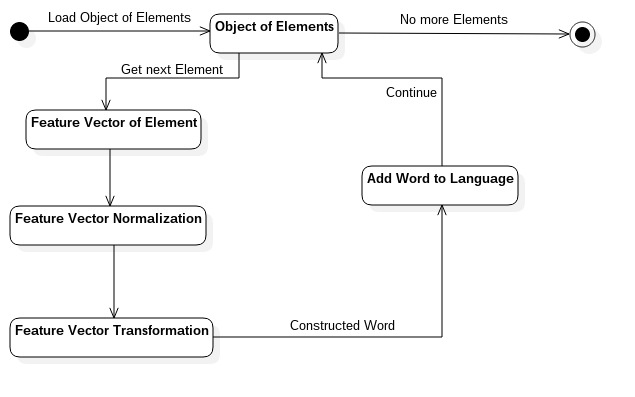
\includegraphics[width=1.0\textwidth]{../uml/states/word_transformation.jpg}
    \caption{State chart of Language Transformation}
    \label{fig:transf_state}
\end{figure}

%---------------------------------------------------------------
%---------------------------------------------------------------
\section{Classification Language}\label{sec:lan_theory_class_lan}
Thus far, the method of classifying an element in terms of languages has been defined. This section focuses on the details of the classification process.

In the previous section it was mentioned that to properly classify a word to its language, it should be included in that language and should not appear in any other. In other words, the goal in proper classification should be the optimum partitioning of set of all words over alphabet $\Sigma$. The following explains the meaning of optimum partitioning.

%---------------------------------------------------------------
%---------------------------------------------------------------
%---------------------------------------------------------------
\subsection{Optimum Partitioning}\label{sec:lan_theory_class_lan_opt_part}

Recall from definition~\ref{def:myhill} that relation $R_L$ induced by the language $L$ partitions the set of all words $\Sigma^{*}$ into equivvalence classes. In other words, equivalence classes are disjoint sets of words. Thus having an equivalence class which classifies a word to its respective language, could make for a very convenient classification tool.

Let the languages $L_{1}, L_{2} \text{ and } L_{3}$ be obtained from the language transformation. The idea of optimum partitioning is to split all three languages so that they are included in three different equivalence classes. 

The initial, poor, partitioning is illustrated in figure~\ref{fig:eq_classes_small_precision}. The figure presents example of three equivalence classes from possibly many. The language $L_{3}$ is fully and uniquely included in the class $A_{3}$. Language $L_{1}$ partially belongs to all three classes and $L_{2}$ belongs to both $A_{2}$ and $A_{3}$. Moreover, the first issue that should be addressed is the imperfect transformation precision. Namely, the intersection of languages $L_{1}$ and $L_{2}$ is not empty.

\begin{figure}[H]
    \centering
    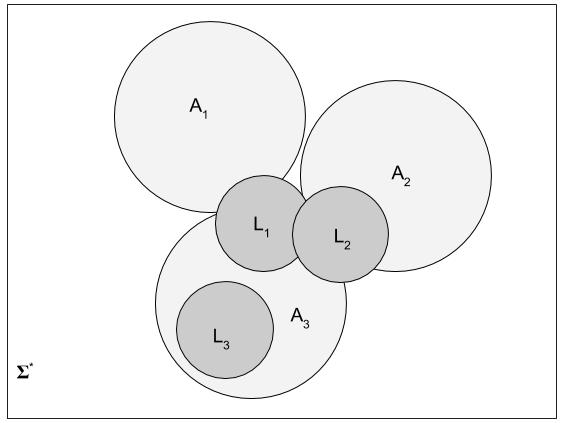
\includegraphics[width=0.7\textwidth]{./images/equivalence_classes_small_pt.jpg}
    \caption{Example of three equivalence classes of Relation Induced by the Classification Language. Languages included in their respective equivalence classes}
    \label{fig:eq_classes_small_precision}
\end{figure}

Figure~\ref{fig:eq_classes_high_precision} shows the same partitioning for higher transformation precision. At this point, all three languages are disjoint but they also share a common class $A_{3}$. Assume that words that fall into $A_{1}$ are considered to be classified to $L_{1}$, similarly with $A_{2}$ for $L_{2}$ and $A_{3}$ for $L_{3}$. Thus having the languages included only partially in their respective classes make for a possible error in classification.

\begin{figure}[H]
    \centering
    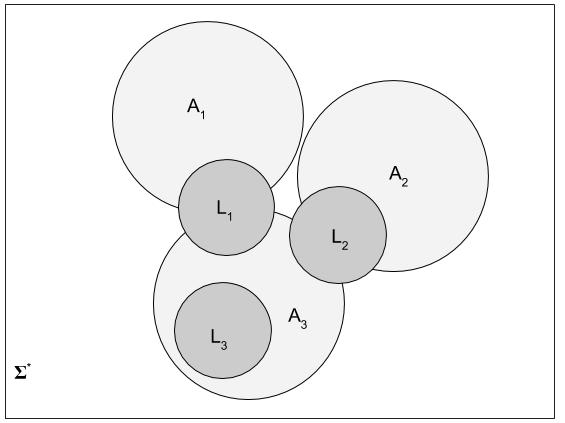
\includegraphics[width=0.7\textwidth]{./images/equivalence_classes_high_pt.jpg}
    \caption{Example of three equivalence classes of Relation Induced by the Classification Language. Languages included in their respective equivalence classes}
    \label{fig:eq_classes_high_precision}
\end{figure}

The next improvement of partitioning is presented in figure~\ref{fig:eq_classes}. All languages are included in only their own respective classes. Words included in class $A_{1}$ will be classified to $L_{1}$. Thus in such a partitioning if words from $L_{1}$ were to be classified to $A_{1}$ then they would be necessarily classified correctly. The same applies to the other two languages. Although, a problem arises when words being classified belong to no particular language and thus are foreign. To maintain good quality of classification process, these words are not supposed to be classified to any of the three equivalence classes. Unfortunately, the classes might be very big, in fact, much bigger than the languages. Thus there are possibly many words that do not describe any particular object, which might be incorrectly classified as one. 

\begin{figure}[H]
    \centering
    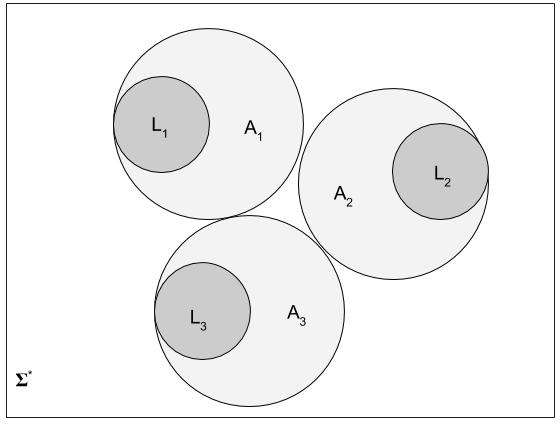
\includegraphics[width=0.7\textwidth]{./images/equivalence_classes.jpg}
    \caption{Example of three equivalence classes of Relation Induced by the Classification Language. Languages included in their respective equivalence classes}
    \label{fig:eq_classes}
\end{figure}

Finally, the figure~\ref{fig:eq_classes_ideal} presents the example of ideal partitioning for three languages. The space of classes and languages are equal, thus all words will be correctly classified.

\begin{figure}[H]
    \centering
    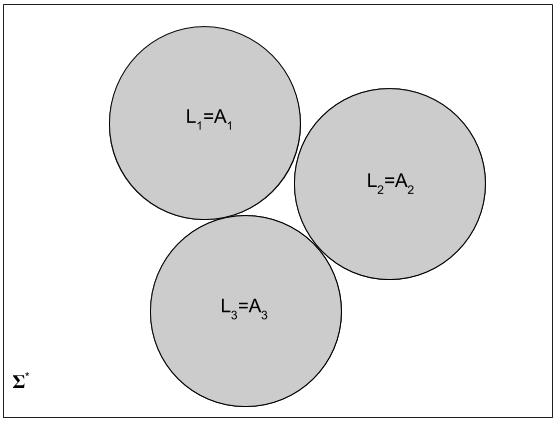
\includegraphics[width=0.7\textwidth]{./images/equivalence_classes_ideal.jpg}
    \caption{Example of three equivalence classes of Relation Induced by the Classification Language. Languages equal to their respective equivalence classes}
    \label{fig:eq_classes_ideal}
\end{figure}

In theory, the problem of optimum partitioning is a problem of constructing a regular language called Classification Language, $L_{C}$ for which equivalence classes of relation induced by $L_{C}$ contain the transformed languages. Ideally, each equivalence class which include and be equal to a single transformed language. The remaining classes will them correspond to the Foreign Language $L_{F}$. 

In practice equivalence classes might be very big and finding ones that perfectly describe a single transformed language can turn out to be a difficult task. Instead, a transformed language could correspond to few equivalence classes, although each class would still correspond to a single language. The intuition behind such procedure is to spread out the transformed languages across the space of all equivalence classes.

%---------------------------------------------------------------
%---------------------------------------------------------------
%---------------------------------------------------------------
\section{Classification Automaton}\label{sec:lan_theory_class_lan_dfa}

The Classification Language is a regular language and thus there exists a Deterministic Finite Automaton (DFA) which accepts it. Moreover, the states of such DFA correspond to the equivalence classes of relation $R_{L_{C}}$. DFA computes a word by returning a final state in which it stopped after the last symbol. Thus, now it is possible to built a classifier using merely a single DFA.

The figure~\ref{fig:class_dfa} shows an example automaton which is used to classify words. It is a deterministic finite automaton with four states and two symbols in the alphabet. States correspond to specific transformed languages. State $4$ corresponds to Foreign Language. Let us assume that some feature vector has been transformed into a word: $f \featureTransformationWord{\Sigma} w = bbb$. Computations for word $w$ will end in state $4$ and will be classified as foreign. However if $w = baba$ then the computations will end in state $2$ and the word will be classified to represent an object described in language $L_2$. Notice, that language $L_1$ is included in two states, in other words there are two equivalence classes that include $L_1$.

\begin{figure}[H]
    \centering
    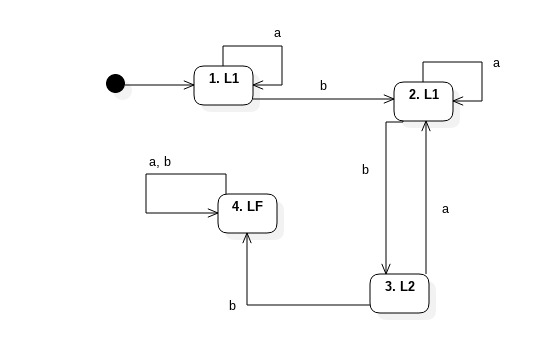
\includegraphics[width=0.7\textwidth]{../uml/states/dfa.jpg}
    \caption{Example of DFA with four states and two symbols. State 1 is the initial state. States $1$ and $2$ correspond to language $L_{1}$, state $3$ to $L_2$ and state $4$ to foreign language $L_F$.}
    \label{fig:class_dfa}
\end{figure}

Finally, building a proper classifier will be equivalent to creating an Classification Automaton $M_{C}$ that minimizes the error of classifying objects in the learning phase. The problem of choosing an optimal number of states corresponding to a transformed languages is to be parametrized and tested empirically.

%---------------------------------------------------------------
%---------------------------------------------------------------
\section{Synthetic Word Generation} \label{sec:lan_theory_synth_word_gen}
 
Let's assume we want to randomly generate words of length $k$ corresponding to some objects. Having fixed number of classes, denoted by $n$ proceed to generate exactly $n$ words representing centres of each class. Then for each such class, start generating uniformly words that are similar to their corresponding centres. Two words can be thought to be \textit{similar} if the ratio of the length and their Hamming distance is reasonably small. Formally the similarity function of two words is defined by the equation:

\begin{equation}
Sr(w,v) = 1 - \frac{H_d(w,v)}{k}
\end{equation}

where $H_d$ is the Hamming distance and $k$ is the length of both words. It is also important to define a similarity threshold~$T_s$ after which we can conclude if two words are similar.

For example, for two words~$w~=~10101$~and~$v~=~00101$ the similarity $Sr(w, v)$ is equal to $0.8$. Assuming a threshold $T_s = 0.7$, we can conclude that these two words are similar. Notice that two equal words are perfectly similar, $S(w,w) = 1$.

The problem still exists in actually defining the threshold for values of $Sr$ for which we can say that two words are similar. For small thresholds, the generated clouds of words might be heavily spread. As a result a chance for any two clouds to be overlapping each other is big. In contrast, when the threshold is big, the clouds will become more clamped and the chance of overlapping is small. On the other hand, the classes constructed by these words, will be defined on a smaller intervals compared to the entire class space. In a result giving us less room to work with.

The intuition can suggest that any two words are similar if their similarity is greater than $0.7$. Although the exact threshold should be experimented with and chosen empirically.

% How about the upper bound of similarity, what if all words generated are the same -> Uniform distribution should cover that



%---------------------------------------------------------------
\chapter{Particle Swarm Optimization}\label{chap:pso}
In the Particle Swarm Optimization (PSO), originated by Eberhart and Kennedy in~\cite{pso_origin}, we look for optimal solution of the problem in the solution space. 

Each solution is called a particle and it consists of the following fields. First of all, the particle stores $fitness$ value which is evaluated by the fitness function, representing the quality of the solution and the best fitness value computed so far. It also stores the position $X_p$ and velocity vector $V_p$ which lets the particle travel through the solution space. Lastly two additional positions called $pbest_p$ and $lbest_p$ are stored. The position in which the particle $p$ reached its best fitness value so far is called $pbest_p$. However, the $lbest_p$ is the position of the best fitness value obtained so far by any other particle in the neighbourhood of particle $p$. The concept of neighbourhood is defined later in this section.

PSO is initialized with random group of particles. It then searches for the optimal solution by updating generations.
In each iteration $t$, the particles are updated by calculating new fitness and velocity which in turn is applied to update new position of the particle. $X_p(t)$ will denote the position of particle $p$ at time $t$, i.e. the $t$-th iteration. Similarly, the velocity vector is denoted by $V_p(t)$.

The PSO will take as input number of states $n$ and number of symbols in alphabet $r$.

Firstly, the general flow of the PSO algorithm is given, then each module is discussed and defined in details.

\begin{center}
    
    \begin{enumerate}
        \item For the input $n$ and $r$, initialize the group of particles.
        
        \item For each particle: \label{itm:pso_iter}
        \begin{enumerate}
            \item Calculate the fitness value, using the fitness function.
            \item Compare the fitness to its best obtained so far, the better value is stored together with $pbest_p$	
            
            \item Update velocity and position.	
            
            \item Find neighbourhood and update $lbest_p$ position.
        \end{enumerate}		
        
        
        
        \item Repeat~\ref{itm:pso_iter}. until an ending criterion is met.
        
        \item Output the best solution	
        
    \end{enumerate}
    
\end{center}

The figure~\ref{fig:pso_state} presents the flow of PSO computations.
\begin{figure}
    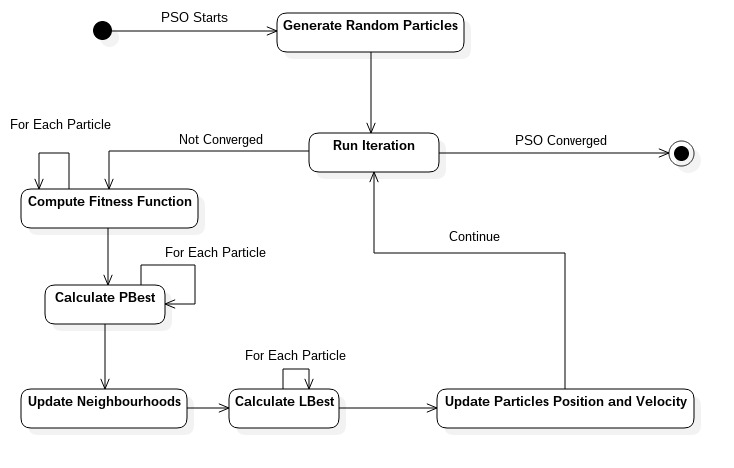
\includegraphics[width=1.0\textwidth]{../uml/states/pso.jpg}
    \caption{State diagram of PSO computations}
    \label{fig:pso_state}
\end{figure}

We now concentrate on describing in details each step of the PSO algorithm. The following part of this section is devoted to illustrating problems associated with the objective of this study and more importantly, methods of solving these problems.


%---------------------------------------------------------------------
%---------------------------------------------------------------------
\section{Representing the solution}
As an input, the PSO algorithm takes number of states $n$ and number of symbols in the alphabet $r$.
Solution that the PSO is trying to find is an automaton. Let us recall that automaton is a system: $A = (Q, \Sigma, \delta, q_0, F)$. In a single PSO instance we assume that a set of states $Q$ and alphabet $\Sigma$ is invariant. 

The position of our particles will be represented by the natural decoding vector of size $n*r$ of an automaton described in section~\ref{sec:auto_dec} with more freedom allowed. Namely, all of the dimensions of the position will take real values in the interval $[0.5, (n+0.5)]$. Whenever we need to encode the automaton back, we simply round up the values, taking the closest integer value. The real number $3.4$ becomes $3$ and $3.5$ becomes 4. Notice that the interval is expanded by the value $0.5$. Such procedure is needed to allow for equal distribution of the first and last states. Namely, the first state will be encoded for values: $[0.5, 1.5]$ and the last state: $[(n-0.5), (n+0.5)]$.

As we may learn further in the article, the method of updating the particle will make a good use of continuous interval. On the other hand, the method of rounding up real numbers, might be vulnerable to error.



%---------------------------------------------------------------------
%---------------------------------------------------------------------
\section{Initialization}
In order to initialize the PSO algorithm, we must first decide on the size of the swarm (i.e. the number of particles). The swarm will be a static group, meaning that the size will not change through out the computations of a single PSO instance. The size should then be a constant value, in terms of an automaton given at the time. We propose that the size of the swarm should be proportional to the size of the automaton. To be precise, the swarm size is equal to the size of the automaton times a constant $c_P$ called a $population$ factor.

Further, we must initialize particle's position. Let us recall that the dimension of the search space is defined by the size of an automaton, namely $(n*r)$, where $n$ is the number of states and $r$ is the number of symbols in the alphabet. Each dimension is taking a real value in the range $[0.5, (n+0.5)]$. Thus, we proceed to generate random position in the given range.

The initial velocities will be generated from the range $[-n,n]$. It is also crucial to define a maximum change in position that one particle can take during a single iteration. For this purpose the constant $v_{max}$ is defined that prevents the particle from travelling in any dimension further than $v_{max}$ units. The maximum change is defined by the equation 

\begin{equation}
    v_{max} = (\frac{n}{2})c_{v}
\end{equation}
where $c_{v}$ is a constant $speed$ factor and $v_{max} \leq n$.

In all cases uniform distribution is used for random number generation.

%---------------------------------------------------------------------
%---------------------------------------------------------------------
\section{Fitness Function}\label{sec:fitness}
Recall that each state in the DFA will correspond to some transformed language and thus will classify a word accordingly. A language can correspond to many states. 

The state correspondence is to be determined prior to starting PSO. The fitness function as an input will take a set of words. Each word belongs to some transformed language which representing an object. Such word will be computed by each encoded particle (i.e. DFA) and thus classified to some language. Fitness function for each particle will then determine the error rate between correctly and incorrectly classified words.

%---------------------------------------------------------------------
%---------------------------------------------------------------------
\section{Updating the particle}


% Naive approach

%The naive approach of updating the particles' positions was proposed in the original PSO %algorithm~\cite{pso_origin}.

%\begin{equation}
%		V_p(t+1) = V_p(t) + c_1 * \mu_1 *(pbest_p - X_p(t)) + c_2 * \mu_2 *(lbest_p - X_p(t))
%	\end{equation}
%
%	\begin{equation}
%		X_p(t+1) = X_p(t) + V_p(t)
%	\end{equation}
%	where:\\
%	$c_1, c_2$ are the constant learning factors.\\
%	$\mu_1, \mu_2$ are random numbers in the range [0,1]. {\color{red} TODO What %distribution function - uniform ?} \\



The following method of updating the particles has its origins in the Standard Particle Swarm Optimization version 2011 presented in~\cite{pso_11}

Let $G_p(t)$ be the centre of gravity of the three points:
\begin{enumerate}
    \item Current position. \\
    $X_p(t)$
    
    \item Point a bit beyond $pbest_p$. \\
    $Y_{p1}(t) = c*(pbest_p-X_p(t))$
    
    \item Point a bit beyond $lbest_p$. \\
    $Y_{p2}(t) = c*(lbest_p-X_p(t))$
    
\end{enumerate}

The constant $c = \frac{1}{2} + ln(2)$ called a learning factor, together with the inertia parameter that weights the particle's velocity $\omega = \frac{1}{2 * ln(2)}$ used in further equations, was proposed by Clerc in~\cite{pso_anal}.

Formally $G_p(t)$ it is defined by the following formula 
\begin{equation}
    G_p(t) = \frac{X_p(t) + Y_{p1}(t) + Y_{p2}(t)} {3}
\end{equation}

We now define a random point $X^{'}_p$ in the hypersphere
\begin{center}
    $\mathcal{H}_p(G_p, d(G_p, X_p))$ 
\end{center}
of centre $G_p$ and of radius $d(G_p, X_p)$ where the function $d$ is an euclidean distance between two points. The time $t$ has been omitted for simplicity.

The velocity update is computed by
\begin{equation}
    V_p(t+1) = \omega * V_p(t) + X^{'}_p(t) - X_p(t)
\end{equation}
Thus the position is updated by the equation

\begin{equation}
    X_p(t+1) = \omega * V_p(t) + X^{'}_p(t)
\end{equation}

% Exploitation vs Exploration

%This method of updating the particles grants adequate definitions for $exploitation$ and $exploration$. Namely the exploitation occurs when $X_p(t+1)$ is inside atleast one hypersphere $\mathcal{H}_q$, otherwise we recognize exploration.


% Interval confinement
It may happen that the particle might leave the search space, in means that the particle lies outside the acceptable interval. If that happens we generally try to lead the particle back to its right course. For each dimension $x_{d} \in X_p$ that lies  outside the acceptable interval we apply the following:

\[
x_{d} \notin [x_{min}, x_{max}] \Rightarrow \left \{
\begin{array}{ll}
v_{d} = 0 \\
x_d < x_{min} \Rightarrow x_d = x_{min} \\
x_d > x_{max} \Rightarrow x_d = x_{max}
\end{array}
\right.
\]

This means that the corresponding dimension of velocity vector $v_d \in V_p$ is zeroed and the position is bound to the edge of the interval.


%---------------------------------------------------------------------
%---------------------------------------------------------------------
\section{Neighbourhood}
The neighbourhood system is defined by grouping the swarm into clusters. Cluster evaluation methods are deployed to estimate the number of clusters $k$ that a data set should be grouped with. Having the knowledge of data distortion, the data is then clustered into $k$ clusters, where each cluster represents a single neighbourhood. K-means algorithm is used to compute the clustering and McClain-Rao index to estimate the optimal clustering. The following formulates the algorithm for neighbourhood update.

\begin{enumerate}
    \item Evaluate number of clusters in the swarm using the McClian-Rao index. Denote that number by $k$.
    \item Group the swarm into $k$ clusters using k-means algorithm.
    \item Each cluster represents a single neighbourhood.
\end{enumerate}


%---------------------------------------------------------------------
%---------------------------------------------------------------------
\section{Ending criteria}
The computation finishes after $t_{max}$ iterations or after finding a satisfactory solution which is bounded by $F_{max} \in [0,1]$, where value 1 corresponds to trying to find the best automaton.

%---------------------------------------------------------------
\chapter{Classifier}\label{chap:classification}

In this chapter, each step of building the classifier is summarized and explicitly described.

%---------------------------------------------------------------
%---------------------------------------------------------------
\section{Building the Classifier}\label{sec:classification_transf_step}
Given the input set of objects, the first step is to transform each object into a language. Transformation step also included choosing a proper number of symbols in the alphabet. The transformation precision is to be selected empirically.

The next step includes selecting the correspondence between states and transformed languages. Together with input labeled data, the classifier will ask to select number of states that will correspond to a specific label. Notice that each label might take different number of states. Similarly, number of states for foreign elements will also be selected. The correspondence is also selected empirically.

Thus far, the alphabet and set of states have been chosen. Set of languages have been transformed and the correspondence between them and states have been established. The process now turns to the stochastic algorithm of PSO. It will look for the most optimal automaton which minimizes the error of incorrectly classified words.


%---------------------------------------------------------------
\chapter{Experiments}\label{chap:experiments}



%%%
%
% Mutual Similarities. Alphabet 24
%
%%%
\begin{figure}[H]
    \CenterFloatBoxes
    \begin{floatrow}
        
        \ttabbox
        {
            \centering
            \setlength{\tabcolsep}{10pt}
            \renewcommand{\arraystretch}{1.5}
            \begin{tabular}{|P{1.0cm} || P{0.6cm} | P{0.6cm} | P{0.6cm} | P{0.6cm} | P{0.6cm} | P{0.6cm} |P{0.6cm} | P{0.6cm} |P{0.6cm} | P{0.6cm}|}
                \hline
                $Sim$ & L0 & L1 & L2 & L3 & L4 & L5 & L6 & L7 & L8 & L9\\
                \hline
                \hline
                L0 &1&0.38&0.37&0.34&0.33&0.33&0.45&0.34&0.45&0.38\\
                \hline
                L1 &0.38&1&0.35&0.34&0.33&0.36&0.39&0.38&0.4&0.36\\
                \hline
                L2 &0.34&0.31&1&0.36&0.33&0.34&0.35&0.36&0.33&0.34\\
                \hline
                L3 &0.33&0.33&0.38&1&0.35&0.4&0.34&0.36&0.34&0.35\\
                \hline
                L4 &0.31&0.33&0.33&0.34&1&0.34&0.35&0.38&0.32&0.38\\
                \hline
                L5 &0.31&0.34&0.35&0.4&0.35&1&0.34&0.35&0.35&0.35\\
                \hline
                L6 &0.45&0.37&0.36&0.34&0.37&0.33&1&0.35&0.41&0.39\\
                \hline
                L7 &0.32&0.36&0.37&0.37&0.37&0.35&0.35&1&0.36&0.4\\
                \hline
                L8 &0.44&0.39&0.36&0.36&0.34&0.35&0.41&0.37&1&0.4\\
                \hline
                L9 &0.36&0.33&0.35&0.35&0.39&0.33&0.38&0.41&0.39&1\\
                \hline
            \end{tabular}
        }
        {\caption{Mutual Similarity of languages. Alphabet size: 24}
        \label{fig:tab_similarity}}
        %\ffigbox
        %  {\includegraphics[width=0.35\textwidth]%{images/automaton_example.jpg}}
        %  {\caption{Example of Automaton %A}\label{fig:automaton_ex}}
        %\killfloatstyle
        
    \end{floatrow}
\end{figure}


%%%
%
% Mutual Similarities. Alphabet 12
%
%%%
\begin{figure}[H]
    \CenterFloatBoxes
    \begin{floatrow}
        
        \ttabbox
        {
            \centering
            \setlength{\tabcolsep}{10pt}
            \renewcommand{\arraystretch}{1.5}
            \begin{tabular}{|P{1.0cm} || P{0.6cm} | P{0.6cm} | P{0.6cm} | P{0.6cm} | P{0.6cm} | P{0.6cm} |P{0.6cm} | P{0.6cm} |P{0.6cm} | P{0.6cm}|}
                \hline
                $Sim$ & L0 & L1 & L2 & L3 & L4 & L5 & L6 & L7 & L8 & L9\\
                \hline
                \hline
                L0 &1&0.51&0.48&0.45&0.44&0.45&0.57&0.45&0.58&0.5\\ 
                \hline 
                L1 &0.51&1&0.45&0.44&0.43&0.46&0.5&0.47&0.53&0.47\\ 
                \hline 
                L2 &0.44&0.41&1&0.47&0.43&0.44&0.45&0.47&0.44&0.44\\ 
                \hline 
                L3 &0.43&0.42&0.5&1&0.46&0.52&0.43&0.47&0.45&0.46\\ 
                \hline 
                L4 &0.41&0.41&0.43&0.45&1&0.45&0.45&0.49&0.43&0.5\\ 
                \hline 
                L5 &0.41&0.44&0.45&0.52&0.45&1&0.43&0.45&0.46&0.46\\ 
                \hline 
                L6 &0.57&0.48&0.47&0.43&0.48&0.44&1&0.45&0.53&0.5\\ 
                \hline 
                L7 &0.41&0.45&0.48&0.48&0.47&0.44&0.45&1&0.46&0.51\\ 
                \hline 
                L8 &0.56&0.52&0.47&0.48&0.45&0.47&0.53&0.48&1&0.52\\ 
                \hline 
                L9 &0.47&0.43&0.46&0.47&0.52&0.44&0.49&0.55&0.51&1 \\
                \hline
            \end{tabular}
        }
        {\caption{Mutual Similarity of languages. Alphabet size: 12}
            \label{fig:tab_similarity}}
        %\ffigbox
        %  {\includegraphics[width=0.35\textwidth]%{images/automaton_example.jpg}}
        %  {\caption{Example of Automaton %A}\label{fig:automaton_ex}}
        %\killfloatstyle
        
    \end{floatrow}
\end{figure}



%%%
%
% Mutual Similarities. Alphabet 6
%
%%%
\begin{figure}[H]
    \CenterFloatBoxes
    \begin{floatrow}
        
        \ttabbox
        {
            \centering
            \setlength{\tabcolsep}{10pt}
            \renewcommand{\arraystretch}{1.5}
            \begin{tabular}{|P{1.0cm} || P{0.6cm} | P{0.6cm} | P{0.6cm} | P{0.6cm} | P{0.6cm} | P{0.6cm} |P{0.6cm} | P{0.6cm} |P{0.6cm} | P{0.6cm}|}
                \hline
                $Sim$ & L0 & L1 & L2 & L3 & L4 & L5 & L6 & L7 & L8 & L9\\
                \hline
                \hline
                L0 &1&0.67&0.65&0.61&0.62&0.63&0.75&0.61&0.79&0.68\\ 
                \hline
                L1 &0.68&1&0.59&0.58&0.58&0.6&0.65&0.62&0.69&0.62\\ 
                \hline
                L2 &0.59&0.57&1&0.64&0.57&0.58&0.6&0.62&0.61&0.59\\ 
                \hline
                L3 &0.58&0.56&0.67&1&0.61&0.7&0.56&0.63&0.62&0.64\\ 
                \hline
                L4 &0.56&0.55&0.58&0.6&1&0.59&0.59&0.64&0.6&0.67\\ 
                \hline
                L5 &0.54&0.57&0.59&0.68&0.59&1&0.58&0.6&0.63&0.62\\ 
                \hline
                L6 &0.75&0.64&0.64&0.57&0.65&0.62&1&0.59&0.72&0.67\\ 
                \hline
                L7 &0.57&0.58&0.64&0.65&0.62&0.58&0.59&1&0.63&0.68\\ 
                \hline
                L8 &0.75&0.68&0.65&0.64&0.65&0.65&0.7&0.66&1&0.72\\ 
                \hline
                L9 &0.65&0.58&0.63&0.63&0.72&0.61&0.63&0.72&0.7&1 \\
                \hline
            \end{tabular}
        }
        {\caption{Mutual Similarity of languages. Alphabet size: 6}
            \label{fig:tab_similarity}}
        %\ffigbox
        %  {\includegraphics[width=0.35\textwidth]%{images/automaton_example.jpg}}
        %  {\caption{Example of Automaton %A}\label{fig:automaton_ex}}
        %\killfloatstyle
        
    \end{floatrow}
\end{figure}


\section{Object Transformation}

TODO Analysis: Alphabet size vs feature vector dimension.
24 symbols seems to be a good chose. coincidence ? I dont think so mate

\begin{figure}[H]
    \caption{Similarity of Transformed Languages. Features 24, 12 and 6}
    \label{fig:lang_sim}
    
    \setPlotStyle
    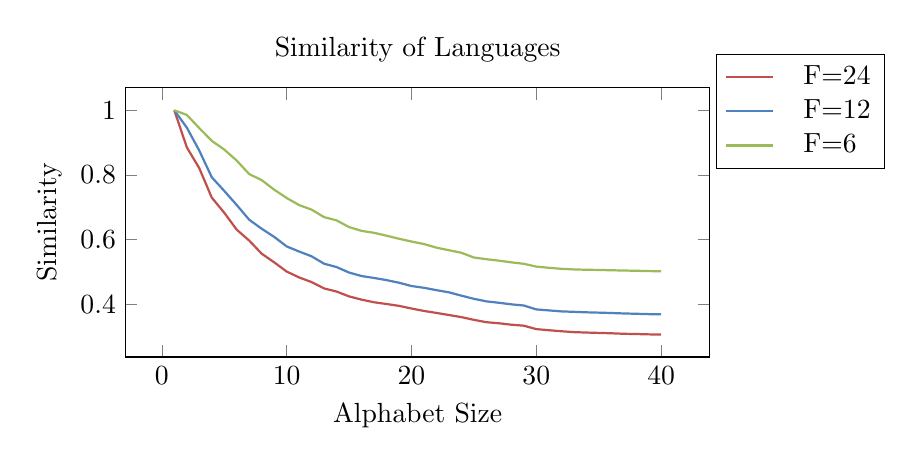
\begin{tikzpicture}
    
    \begin{groupplot}[group style={group size= 1 by 1,
        vertical sep=50pt, horizontal sep=40pt}, 
    height=5cm,
    width=9cm,
    ylabel=Similarity,
    xlabel=Alphabet Size,
    legend cell align=left, 
    legend columns=1,
    legend style={
        at={(1.3, 0.7)}, 
        anchor=south east, 
        column sep=2ex
    }
    ]
    
    \nextgroupplot[title=Similarity of Languages]
    
    % RECONS_C4_CL4
    \addplot[color=rred, thick] coordinates {
        (1, 1.0)
        (2, 0.885624)
        (3, 0.820992)
        (4, 0.730032)
        (5, 0.683266)
        (6, 0.630893)
        (7, 0.597193)
        (8, 0.556699)
        (9, 0.530009)
        (10, 0.501454)
        (11, 0.483245)
        (12, 0.468839)
        (13, 0.449223)
        (14, 0.439578)
        (15, 0.424618)
        (16, 0.414595)
        (17, 0.40647)
        (18, 0.40111)
        (19, 0.395343)
        (20, 0.387143)
        (21, 0.379669)
        (22, 0.373499)
        (23, 0.367048)
        (24, 0.360526)
        (25, 0.352155)
        (26, 0.344844)
        (27, 0.341559)
        (28, 0.3371)
        (29, 0.334055)
        (30, 0.323485)
        (31, 0.320073)
        (32, 0.316891)
        (33, 0.314173)
        (34, 0.312831)
        (35, 0.31173)
        (36, 0.310632)
        (37, 0.308987)
        (38, 0.308271)
        (39, 0.307231)
        (40, 0.306493)
    };
    
    \addplot[color=bblue, thick] coordinates {
        (1, 1)
        (2, 0.946593)
        (3, 0.875411)
        (4, 0.793013)
        (5, 0.750825)
        (6, 0.707227)
        (7, 0.661645)
        (8, 0.633788)
        (9, 0.608713)
        (10, 0.579212)
        (11, 0.563333)
        (12, 0.548493)
        (13, 0.525693)
        (14, 0.515291)
        (15, 0.49837)
        (16, 0.487564)
        (17, 0.481635)
        (18, 0.474955)
        (19, 0.466881)
        (20, 0.456707)
        (21, 0.451241)
        (22, 0.443928)
        (23, 0.437209)
        (24, 0.426873)
        (25, 0.417163)
        (26, 0.409276)
        (27, 0.40494)
        (28, 0.400052)
        (29, 0.396438)
        (30, 0.384415)
        (31, 0.381331)
        (32, 0.378308)
        (33, 0.376923)
        (34, 0.375386)
        (35, 0.374406)
        (36, 0.373315)
        (37, 0.371841)
        (38, 0.370896)
        (39, 0.369772)
        (40, 0.369068)
    };
    
    \addplot[color=ggreen, mark=X, thick] coordinates {
        (1, 1)
        (2, 0.985716)
        (3, 0.945022)
        (4, 0.905648)
        (5, 0.878641)
        (6, 0.844539)
        (7, 0.802885)
        (8, 0.784123)
        (9, 0.754583)
        (10, 0.728829)
        (11, 0.706925)
        (12, 0.692846)
        (13, 0.669685)
        (14, 0.659658)
        (15, 0.638983)
        (16, 0.627259)
        (17, 0.621248)
        (18, 0.612334)
        (19, 0.602844)
        (20, 0.594297)
        (21, 0.586517)
        (22, 0.575423)
        (23, 0.567364)
        (24, 0.559515)
        (25, 0.544873)
        (26, 0.539592)
        (27, 0.535175)
        (28, 0.529889)
        (29, 0.525394)
        (30, 0.516758)
        (31, 0.513072)
        (32, 0.5099)
        (33, 0.508012)
        (34, 0.507009)
        (35, 0.506436)
        (36, 0.50542)
        (37, 0.50464)
        (38, 0.503842)
        (39, 0.502863)
        (40, 0.502346)
    };
    
    \addlegendentry{F=24}
    \addlegendentry{F=12}
    \addlegendentry{F=6}
    
    \end{groupplot}
    
    \end{tikzpicture}
    
\end{figure}




%%%
%
% PSO For different classes
%
%%%
\begin{figure}[H]
    \caption{TODO: Classifier Quality for 1, 2, .., 10 classes. Object count in each class: 900. States per native class: 2. States per foreign class: twice as less as all natives. Distinct-Testing}
    \label{fig:lang_sim}
    
    \setPlotStyle
    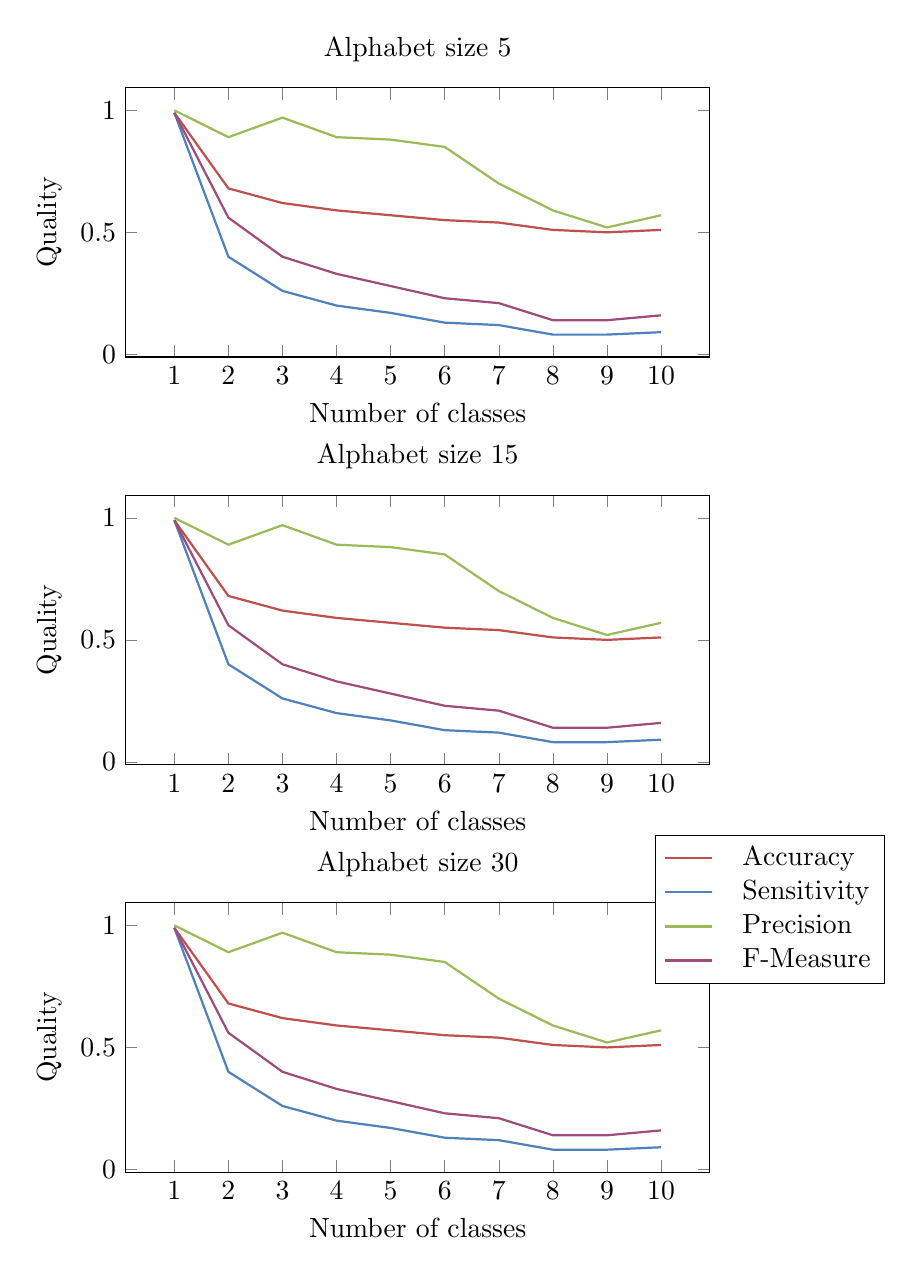
\begin{tikzpicture}
    
    \begin{groupplot}[group style={group size= 1 by 3,
        vertical sep=50pt, horizontal sep=40pt}, 
    height=5cm,
    width=9cm,
    ylabel=Quality,
    xtick={1,2,3,4,5,6,7,8,9,10},
    xlabel=Number of classes,
    legend cell align=left, 
    legend columns=1,
    legend style={
        at={(1.3, 0.7)}, 
        anchor=south east, 
        column sep=2ex
    }
    ]
    
    \nextgroupplot[title=Alphabet size 5]
    
    % ACCURACY
    \addplot[color=rred, thick] coordinates {
        (1, 0.99)
        (2, 0.68)
        (3, 0.62)
        (4, 0.59)
        (5, 0.57)
        (6, 0.55)
        (7, 0.54)
        (8, 0.51)
        (9, 0.50)
        (10, 0.51)
    };
    
    % SENSITIVITY
    \addplot[color=bblue, thick] coordinates {
        (1, 0.99)
        (2, 0.40)
        (3, 0.26)
        (4, 0.2)
        (5, 0.17)
        (6, 0.13)
        (7, 0.12)
        (8, 0.081)
        (9, 0.081)
        (10, 0.091)
    };
    % PRECISION
    \addplot[color=ggreen, mark=X, thick] coordinates {
        (1, 1.00)
        (2, 0.89)
        (3, 0.97)
        (4, 0.89)
        (5, 0.88)
        (6, 0.85)
        (7, 0.70)
        (8, 0.59)
        (9, 0.52)
        (10, 0.57)
    };
    % F-MEASURE
    \addplot[color=ppurple, mark=X, thick] coordinates {
        (1, 0.99)
        (2, 0.56)
        (3, 0.40)
        (4, 0.33)
        (5, 0.28)
        (6, 0.23)
        (7, 0.21)
        (8, 0.14)
        (9, 0.14)
        (10, 0.16)
    };
    
    \nextgroupplot[title=Alphabet size 15]
    
    % ACCURACY
    \addplot[color=rred, thick] coordinates {
        (1, 0.99)
        (2, 0.68)
        (3, 0.62)
        (4, 0.59)
        (5, 0.57)
        (6, 0.55)
        (7, 0.54)
        (8, 0.51)
        (9, 0.50)
        (10, 0.51)
    };
    
    % SENSITIVITY
    \addplot[color=bblue, thick] coordinates {
        (1, 0.99)
        (2, 0.40)
        (3, 0.26)
        (4, 0.2)
        (5, 0.17)
        (6, 0.13)
        (7, 0.12)
        (8, 0.081)
        (9, 0.081)
        (10, 0.091)
    };
    % PRECISION
    \addplot[color=ggreen, mark=X, thick] coordinates {
        (1, 1.00)
        (2, 0.89)
        (3, 0.97)
        (4, 0.89)
        (5, 0.88)
        (6, 0.85)
        (7, 0.70)
        (8, 0.59)
        (9, 0.52)
        (10, 0.57)
    };
    % F-MEASURE
    \addplot[color=ppurple, mark=X, thick] coordinates {
        (1, 0.99)
        (2, 0.56)
        (3, 0.40)
        (4, 0.33)
        (5, 0.28)
        (6, 0.23)
        (7, 0.21)
        (8, 0.14)
        (9, 0.14)
        (10, 0.16)
    };

    \nextgroupplot[title=Alphabet size 30]
    
    % ACCURACY
    \addplot[color=rred, thick] coordinates {
        (1, 0.99)
        (2, 0.68)
        (3, 0.62)
        (4, 0.59)
        (5, 0.57)
        (6, 0.55)
        (7, 0.54)
        (8, 0.51)
        (9, 0.50)
        (10, 0.51)
    };
    
    % SENSITIVITY
    \addplot[color=bblue, thick] coordinates {
        (1, 0.99)
        (2, 0.40)
        (3, 0.26)
        (4, 0.2)
        (5, 0.17)
        (6, 0.13)
        (7, 0.12)
        (8, 0.081)
        (9, 0.081)
        (10, 0.091)
    };
    % PRECISION
    \addplot[color=ggreen, mark=X, thick] coordinates {
        (1, 1.00)
        (2, 0.89)
        (3, 0.97)
        (4, 0.89)
        (5, 0.88)
        (6, 0.85)
        (7, 0.70)
        (8, 0.59)
        (9, 0.52)
        (10, 0.57)
    };
    % F-MEASURE
    \addplot[color=ppurple, mark=X, thick] coordinates {
        (1, 0.99)
        (2, 0.56)
        (3, 0.40)
        (4, 0.33)
        (5, 0.28)
        (6, 0.23)
        (7, 0.21)
        (8, 0.14)
        (9, 0.14)
        (10, 0.16)
    };
    
    \addlegendentry{Accuracy}
    \addlegendentry{Sensitivity}
    \addlegendentry{Precision}
    \addlegendentry{F-Measure}
    
    \end{groupplot}

    \end{tikzpicture}
    
\end{figure}









%%%
%
% PSO For different classes
%
%%%
\begin{figure}[H]
    \caption{TODO: Classifier Quality for 1, 2, .., 10 classes. Object count in each class: 900. States per native class: 2. States per foreign class: as many as all natives. Distinct-Testing}
    \label{fig:lang_sim}
    
    \setPlotStyle
    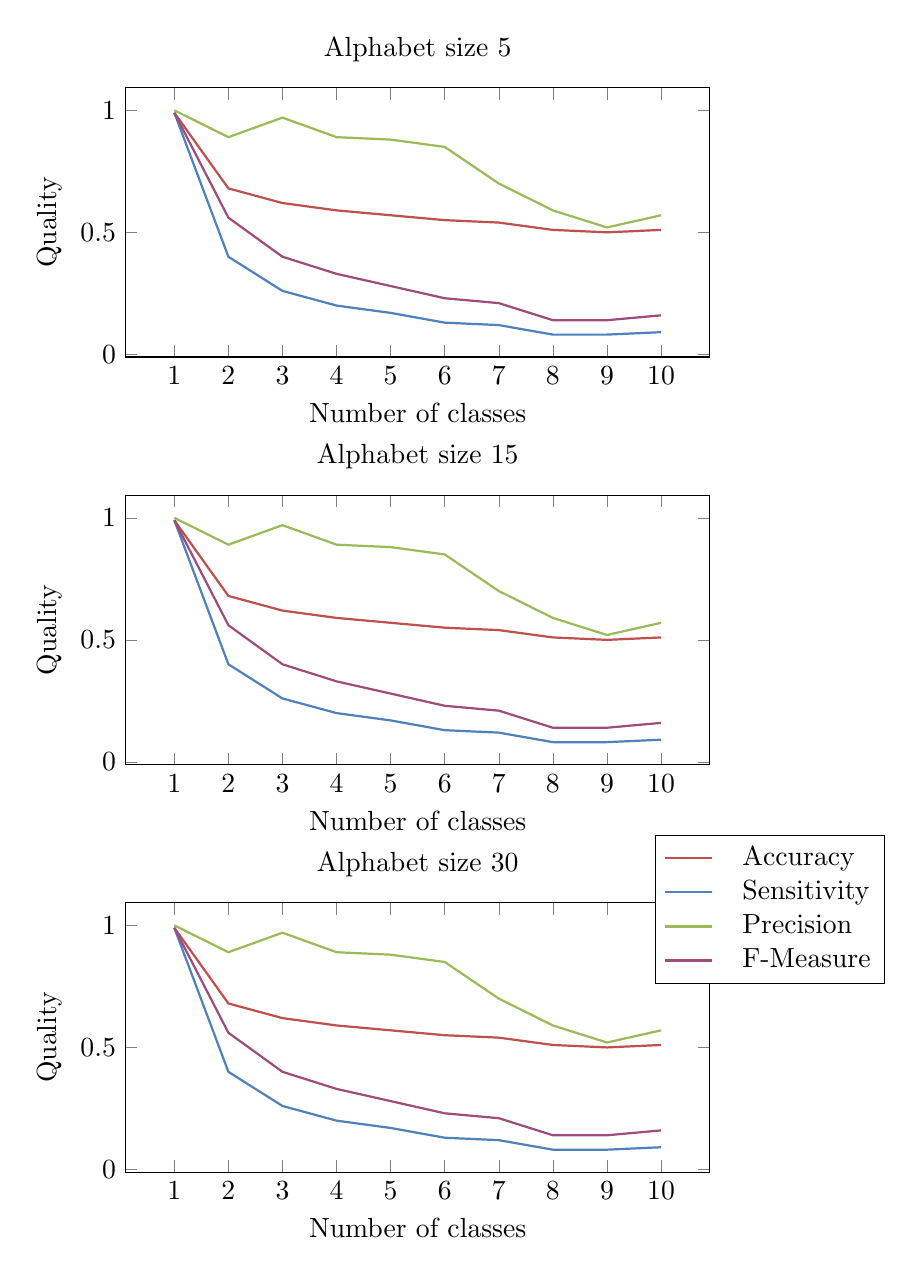
\begin{tikzpicture}
    
    \begin{groupplot}[group style={group size= 1 by 3,
        vertical sep=50pt, horizontal sep=40pt}, 
    height=5cm,
    width=9cm,
    ylabel=Quality,
    xtick={1,2,3,4,5,6,7,8,9,10},
    xlabel=Number of classes,
    legend cell align=left, 
    legend columns=1,
    legend style={
        at={(1.3, 0.7)}, 
        anchor=south east, 
        column sep=2ex
    }
    ]
    
    \nextgroupplot[title=Alphabet size 5]
    
    % ACCURACY
    \addplot[color=rred, thick] coordinates {
        (1, 0.99)
        (2, 0.68)
        (3, 0.62)
        (4, 0.59)
        (5, 0.57)
        (6, 0.55)
        (7, 0.54)
        (8, 0.51)
        (9, 0.50)
        (10, 0.51)
    };
    
    % SENSITIVITY
    \addplot[color=bblue, thick] coordinates {
        (1, 0.99)
        (2, 0.40)
        (3, 0.26)
        (4, 0.2)
        (5, 0.17)
        (6, 0.13)
        (7, 0.12)
        (8, 0.081)
        (9, 0.081)
        (10, 0.091)
    };
    % PRECISION
    \addplot[color=ggreen, mark=X, thick] coordinates {
        (1, 1.00)
        (2, 0.89)
        (3, 0.97)
        (4, 0.89)
        (5, 0.88)
        (6, 0.85)
        (7, 0.70)
        (8, 0.59)
        (9, 0.52)
        (10, 0.57)
    };
    % F-MEASURE
    \addplot[color=ppurple, mark=X, thick] coordinates {
        (1, 0.99)
        (2, 0.56)
        (3, 0.40)
        (4, 0.33)
        (5, 0.28)
        (6, 0.23)
        (7, 0.21)
        (8, 0.14)
        (9, 0.14)
        (10, 0.16)
    };
    
    \nextgroupplot[title=Alphabet size 15]
    
    % ACCURACY
    \addplot[color=rred, thick] coordinates {
        (1, 0.99)
        (2, 0.68)
        (3, 0.62)
        (4, 0.59)
        (5, 0.57)
        (6, 0.55)
        (7, 0.54)
        (8, 0.51)
        (9, 0.50)
        (10, 0.51)
    };
    
    % SENSITIVITY
    \addplot[color=bblue, thick] coordinates {
        (1, 0.99)
        (2, 0.40)
        (3, 0.26)
        (4, 0.2)
        (5, 0.17)
        (6, 0.13)
        (7, 0.12)
        (8, 0.081)
        (9, 0.081)
        (10, 0.091)
    };
    % PRECISION
    \addplot[color=ggreen, mark=X, thick] coordinates {
        (1, 1.00)
        (2, 0.89)
        (3, 0.97)
        (4, 0.89)
        (5, 0.88)
        (6, 0.85)
        (7, 0.70)
        (8, 0.59)
        (9, 0.52)
        (10, 0.57)
    };
    % F-MEASURE
    \addplot[color=ppurple, mark=X, thick] coordinates {
        (1, 0.99)
        (2, 0.56)
        (3, 0.40)
        (4, 0.33)
        (5, 0.28)
        (6, 0.23)
        (7, 0.21)
        (8, 0.14)
        (9, 0.14)
        (10, 0.16)
    };
    
    \nextgroupplot[title=Alphabet size 30]
    
    % ACCURACY
    \addplot[color=rred, thick] coordinates {
        (1, 0.99)
        (2, 0.68)
        (3, 0.62)
        (4, 0.59)
        (5, 0.57)
        (6, 0.55)
        (7, 0.54)
        (8, 0.51)
        (9, 0.50)
        (10, 0.51)
    };
    
    % SENSITIVITY
    \addplot[color=bblue, thick] coordinates {
        (1, 0.99)
        (2, 0.40)
        (3, 0.26)
        (4, 0.2)
        (5, 0.17)
        (6, 0.13)
        (7, 0.12)
        (8, 0.081)
        (9, 0.081)
        (10, 0.091)
    };
    % PRECISION
    \addplot[color=ggreen, mark=X, thick] coordinates {
        (1, 1.00)
        (2, 0.89)
        (3, 0.97)
        (4, 0.89)
        (5, 0.88)
        (6, 0.85)
        (7, 0.70)
        (8, 0.59)
        (9, 0.52)
        (10, 0.57)
    };
    % F-MEASURE
    \addplot[color=ppurple, mark=X, thick] coordinates {
        (1, 0.99)
        (2, 0.56)
        (3, 0.40)
        (4, 0.33)
        (5, 0.28)
        (6, 0.23)
        (7, 0.21)
        (8, 0.14)
        (9, 0.14)
        (10, 0.16)
    };
    
    \addlegendentry{Accuracy}
    \addlegendentry{Sensitivity}
    \addlegendentry{Precision}
    \addlegendentry{F-Measure}
    
    \end{groupplot}
    
    \end{tikzpicture}
    
\end{figure}






%%%
%
% PSO For different classes
%
%%%
\begin{figure}[H]
    \caption{TODO: Classifier Quality for 1, 2, .., 10 classes. Object count in each class: 900. States per native class: 2. States per foreign class: twice as many as all natives. Distinct-Testing}
    \label{fig:lang_sim}
    
    \setPlotStyle
    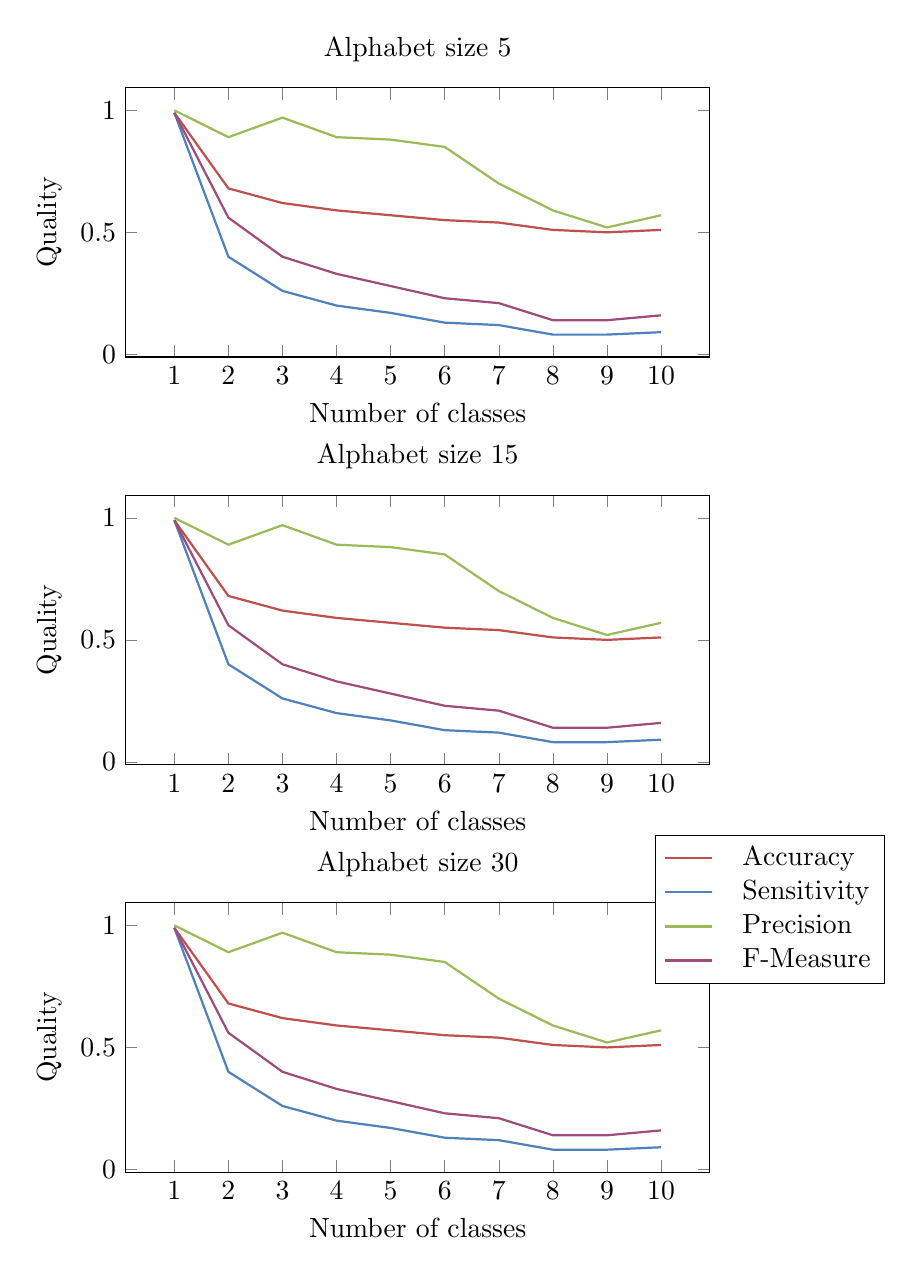
\begin{tikzpicture}
    
    \begin{groupplot}[group style={group size= 1 by 3,
        vertical sep=50pt, horizontal sep=40pt}, 
    height=5cm,
    width=9cm,
    ylabel=Quality,
    xtick={1,2,3,4,5,6,7,8,9,10},
    xlabel=Number of classes,
    legend cell align=left, 
    legend columns=1,
    legend style={
        at={(1.3, 0.7)}, 
        anchor=south east, 
        column sep=2ex
    }
    ]
    
    \nextgroupplot[title=Alphabet size 5]
    
    % ACCURACY
    \addplot[color=rred, thick] coordinates {
        (1, 0.99)
        (2, 0.68)
        (3, 0.62)
        (4, 0.59)
        (5, 0.57)
        (6, 0.55)
        (7, 0.54)
        (8, 0.51)
        (9, 0.50)
        (10, 0.51)
    };
    
    % SENSITIVITY
    \addplot[color=bblue, thick] coordinates {
        (1, 0.99)
        (2, 0.40)
        (3, 0.26)
        (4, 0.2)
        (5, 0.17)
        (6, 0.13)
        (7, 0.12)
        (8, 0.081)
        (9, 0.081)
        (10, 0.091)
    };
    % PRECISION
    \addplot[color=ggreen, mark=X, thick] coordinates {
        (1, 1.00)
        (2, 0.89)
        (3, 0.97)
        (4, 0.89)
        (5, 0.88)
        (6, 0.85)
        (7, 0.70)
        (8, 0.59)
        (9, 0.52)
        (10, 0.57)
    };
    % F-MEASURE
    \addplot[color=ppurple, mark=X, thick] coordinates {
        (1, 0.99)
        (2, 0.56)
        (3, 0.40)
        (4, 0.33)
        (5, 0.28)
        (6, 0.23)
        (7, 0.21)
        (8, 0.14)
        (9, 0.14)
        (10, 0.16)
    };
    
    \nextgroupplot[title=Alphabet size 15]
    
    % ACCURACY
    \addplot[color=rred, thick] coordinates {
        (1, 0.99)
        (2, 0.68)
        (3, 0.62)
        (4, 0.59)
        (5, 0.57)
        (6, 0.55)
        (7, 0.54)
        (8, 0.51)
        (9, 0.50)
        (10, 0.51)
    };
    
    % SENSITIVITY
    \addplot[color=bblue, thick] coordinates {
        (1, 0.99)
        (2, 0.40)
        (3, 0.26)
        (4, 0.2)
        (5, 0.17)
        (6, 0.13)
        (7, 0.12)
        (8, 0.081)
        (9, 0.081)
        (10, 0.091)
    };
    % PRECISION
    \addplot[color=ggreen, mark=X, thick] coordinates {
        (1, 1.00)
        (2, 0.89)
        (3, 0.97)
        (4, 0.89)
        (5, 0.88)
        (6, 0.85)
        (7, 0.70)
        (8, 0.59)
        (9, 0.52)
        (10, 0.57)
    };
    % F-MEASURE
    \addplot[color=ppurple, mark=X, thick] coordinates {
        (1, 0.99)
        (2, 0.56)
        (3, 0.40)
        (4, 0.33)
        (5, 0.28)
        (6, 0.23)
        (7, 0.21)
        (8, 0.14)
        (9, 0.14)
        (10, 0.16)
    };
    
    \nextgroupplot[title=Alphabet size 30]
    
    % ACCURACY
    \addplot[color=rred, thick] coordinates {
        (1, 0.99)
        (2, 0.68)
        (3, 0.62)
        (4, 0.59)
        (5, 0.57)
        (6, 0.55)
        (7, 0.54)
        (8, 0.51)
        (9, 0.50)
        (10, 0.51)
    };
    
    % SENSITIVITY
    \addplot[color=bblue, thick] coordinates {
        (1, 0.99)
        (2, 0.40)
        (3, 0.26)
        (4, 0.2)
        (5, 0.17)
        (6, 0.13)
        (7, 0.12)
        (8, 0.081)
        (9, 0.081)
        (10, 0.091)
    };
    % PRECISION
    \addplot[color=ggreen, mark=X, thick] coordinates {
        (1, 1.00)
        (2, 0.89)
        (3, 0.97)
        (4, 0.89)
        (5, 0.88)
        (6, 0.85)
        (7, 0.70)
        (8, 0.59)
        (9, 0.52)
        (10, 0.57)
    };
    % F-MEASURE
    \addplot[color=ppurple, mark=X, thick] coordinates {
        (1, 0.99)
        (2, 0.56)
        (3, 0.40)
        (4, 0.33)
        (5, 0.28)
        (6, 0.23)
        (7, 0.21)
        (8, 0.14)
        (9, 0.14)
        (10, 0.16)
    };
    
    \addlegendentry{Accuracy}
    \addlegendentry{Sensitivity}
    \addlegendentry{Precision}
    \addlegendentry{F-Measure}
    
    \end{groupplot}
    
    \end{tikzpicture}
    
\end{figure}











\section{PSO}
Native symbols used in the experiments were


%\begin{figure}[H]
%    \caption{Reconstruction. The average accuracy of 10 automata from each class: 4, 6, 10, 15}
%    \label{fig:recons_results}
%    
%    \setPlotStyle
%    \begin{tikzpicture}
%    
%    %%%%%%%%%%%%%%%%%%%%
%    % GROUPPLOT
%    %%%%%%%%%%%%%%%%%%%%
%    
%    \beginGroupPlot
%    
%    
%    \nextgroupplot[title=Class 4,  ylabel=Accuracy]
%    \saveResultsFirst   {0.75}{0.76}{0.76}{0.76}
%    \saveResultsSecond  {0.76}{0.76}{0.76}{0.76}
%    \addBarPlotResults  {C=4}{C=5}
%    
%    \nextgroupplot[title=Class 6]%
%    \saveResultsFirst   {0.77}{0.77}{0.77}{0.77}
%    \saveResultsSecond  {0.77} {0.77}{0.77}{0.77}
%    \addBarPlotResults  {C=4}{C=5}
%    
%    \nextgroupplot[title=Class 10, ylabel=Accuracy]
%    \saveResultsFirst   {0.83}{0.83}{0.83}{0.83}
%    \saveResultsSecond  {0.83}{0.83}{0.83}{0.83}
%    \addBarPlotResults  {C=4}{C=5}
%    
%    
%    \nextgroupplot[title=Class 15]
%    \saveResultsFirst   {0.86}{0.86}{0.86}{0.86}
%    \saveResultsSecond  {0.86}{0.86}{0.86}{0.86}
%    \addBarPlotResults  {C=4}{C=5}
%    %%%%%%%%%%%%%%%%%%%%
%    % LEGEND
%    %%%%%%%%%%%%%%%%%%%%
%    \setPlotLegend
%    
%    \end{groupplot}
%    \end{tikzpicture}
%\end{figure}


%---------------------------------------------------------------
\chapter{Results}\label{chap:results}

%
% HILL CLIMBER RESULTS
%
\section{Classifier Based on Hill Climber}
This section presents results for building classifier based only on Hill Climber. We were trying to catch all pros and cons of building DFA, rather naively, based on one heuristic with no interference in states structure. 

\subsection{Results Layout}
Two sets of graphs are presented. Each of them has 6 plots. Plots represents consecutive classes, from $\langle1;6\rangle$ interval, that we are considering. Single outcome is based on the best fitness function value out of 4 computations performed. In each case we take 550 features vectors per class (including foreign ones). 

First set assumes fixed number of states (chosen intuitively) equal to 35 and varying number of alphabet symbols - even numbers from 2 to 18 (inclusively), which are drawn against 4 measures presented in section \ref{evaluation} i.e. Accuracy, Sensitivity, Precision and F-Measure. 

On the other hand, second set fixes number of symbol in alphabet to 6 and presents the measures values for different number of states: 15, 35, 50, 65, 80, 105, 120, 135, 150. We were trying to observe what happens to our DFA-based classifier if we give him wider collection of states to operate on. In addition size of the alphabet was not chosen randomly - based on first set, in every case 6 symbols works relatively well for all 4 measures.

\subsection{Results Outcomes}


\begin{figure}
% CLASSES: 1
\begin{subfigure}{.5\textwidth}
  \centering
  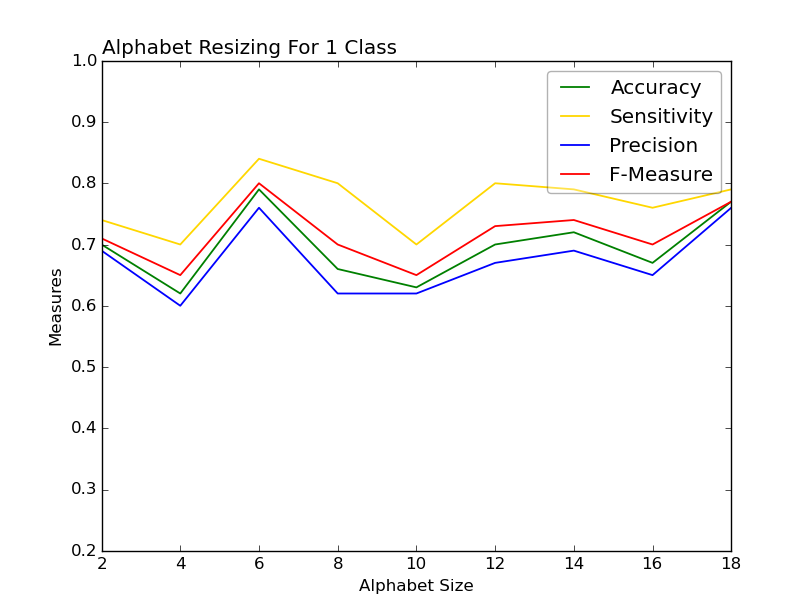
\includegraphics[width=1\linewidth]{images/a_c1_fig.png}
  \label{fig:sfig1}
\end{subfigure}%
\begin{subfigure}{.5\textwidth}
  \centering
  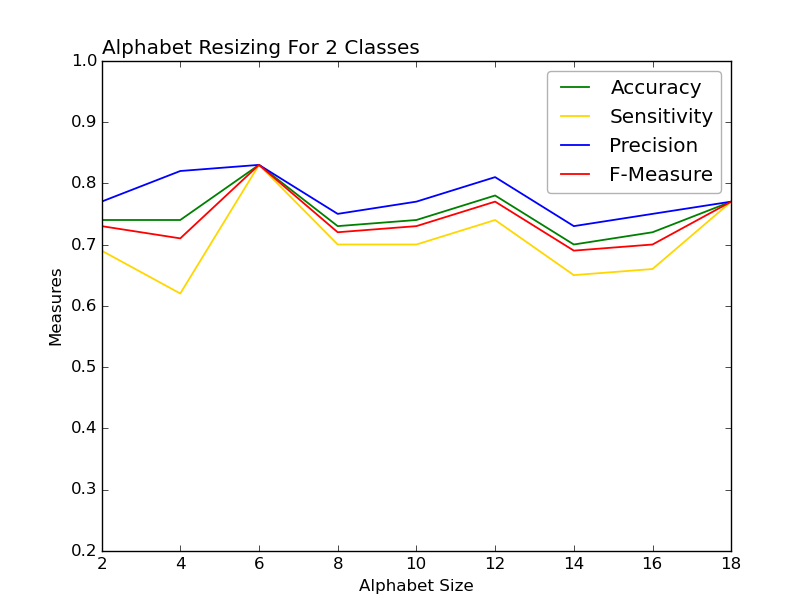
\includegraphics[width=1\linewidth]{images/a_c2_fig.png}
  \label{fig:sfig2}
\end{subfigure}
% CLASSES: 2
\begin{subfigure}{.5\textwidth}
  \centering
  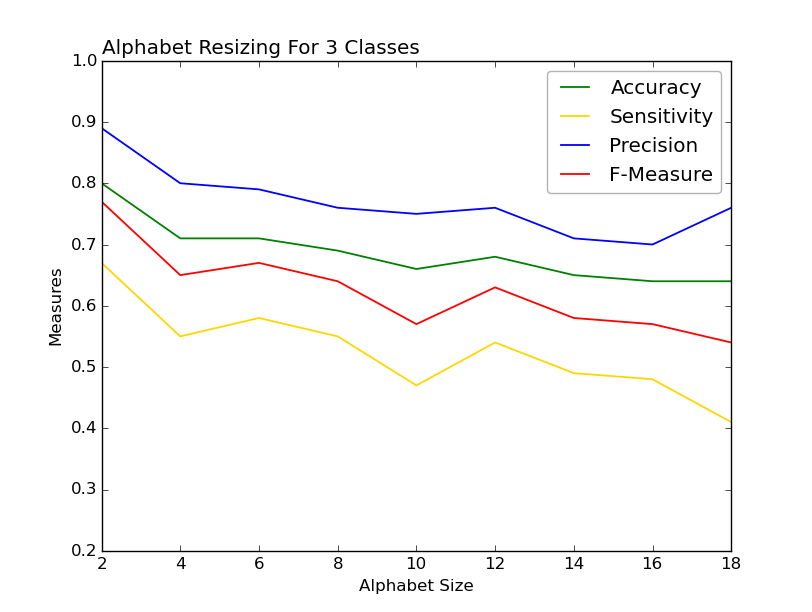
\includegraphics[width=1\linewidth]{images/a_c3_fig.png}
  \label{fig:sfig1}
\end{subfigure}%
\begin{subfigure}{.5\textwidth}
  \centering
  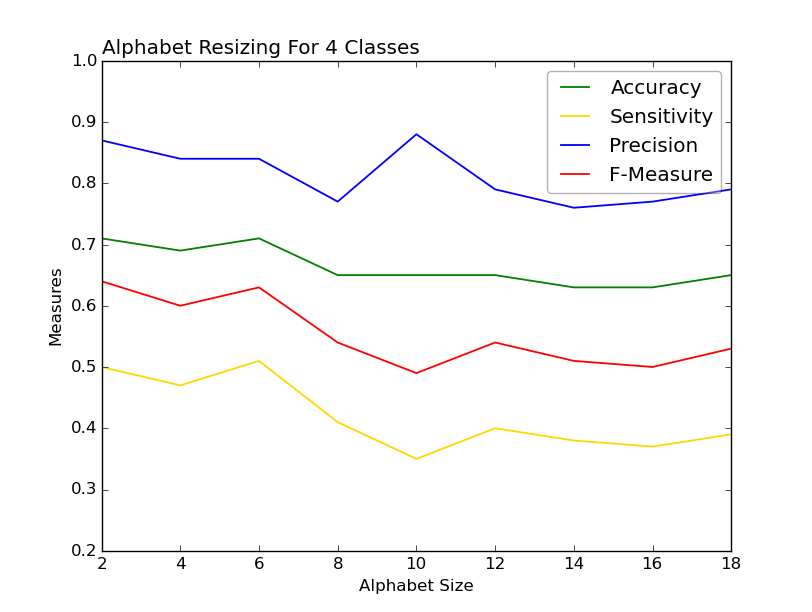
\includegraphics[width=1\linewidth]{images/a_c4_fig.png}
  \label{fig:sfig2}
\end{subfigure}
% CLASSES: 3
\begin{subfigure}{.5\textwidth}
  \centering
  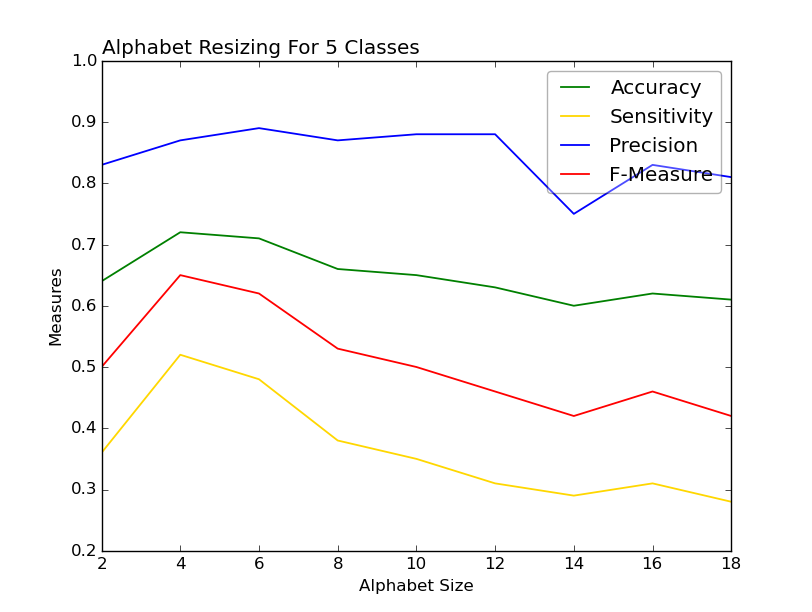
\includegraphics[width=1\linewidth]{images/a_c5_fig.png}
  \label{fig:sfig1}
\end{subfigure}%
\begin{subfigure}{.5\textwidth}
  \centering
  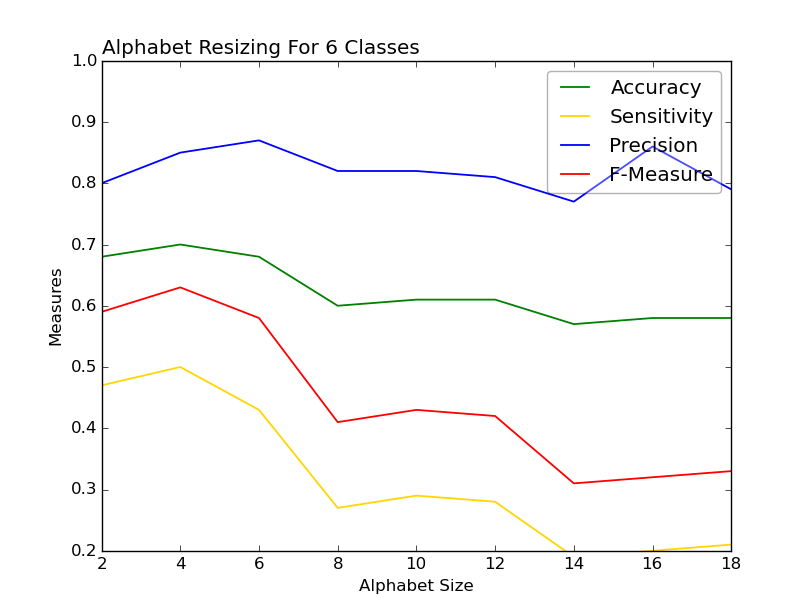
\includegraphics[width=1\linewidth]{images/a_c6_fig.png}
  \label{fig:sfig2}
\end{subfigure}
\caption{Plots depict how various measures react to elevating number of considered classes. Each graph assumes fix number of states (35) and varying number of symbols in alphabet (2-18). Consecutive plots presents increasing number of classes - from 1 to 6.}
\label{fig:fig}
\end{figure}


%---------------------------------------------------------------
\chapter{Domain} \label{chap:domain}
In this chapter the domain of the application is discussed. 

\textbf{Remark:} What should be stress out is that class diagrams presented in this section may not cover all methods needed to implement full functionality. For sure presented methods are necessary, but not always sufficient. Although we were trying to be as precise as we can, they constitutes only a sketch of solution.

The main modules of the application are now presented and briefly explained.

\begin{itemize}
    
    \item 
    {{Classification}} - All the classes responsible for classifying objects.
    \item 
    {{Clustering}} - Method of grouping and cluster evaluation are to be held in this module.
    \item
    {{Word Processing}} - Takes care of word creation.
    \item 
    {{Automaton}} - Describes the Deterministic Finite Automaton, the transition tables and methods of automaton decoding 
    \item 
    {{Math}} - All the mathematical functions related to the application.
    \item 
    {{Utility}} - Functionality which helps to run the project. Logging, system settings, time measurement are examples of what can be included that module.
    \item 
    {{GUI}} - The Graphical User Interface, defines all the classes that construct the interface.
    
\end{itemize}

The remainder of this section will describe these modules in details.

%---------------------------------------------------------------
%---------------------------------------------------------------
\section{Automata}
\begin{figure}[H]
    \centering
    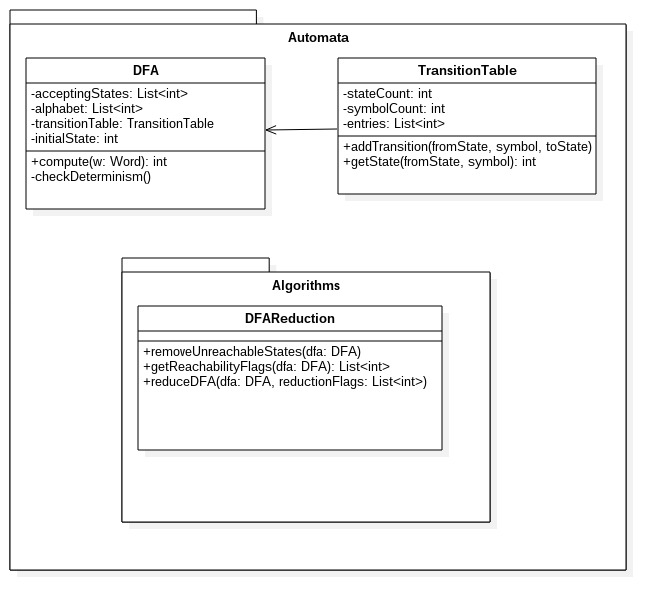
\includegraphics[width=1.0\textwidth]{../uml/classes/automata.jpg}
    \caption{Class diagrams of clustering module}
    \label{fig:automata_class}
\end{figure}


%---------------------------------------------------------------
%---------------------------------------------------------------
\section{Clustering}

The clustering module contains all necessary functionality for analysis of clusters. Figure~\ref{fig:clustering_class} presents few basic classes. \textit{KMeans} constructor takes the maximum iterations and tolerance of convergence. Calling \textit{compute} will start the computation of kmeans algorithm with $k$ clusters for input data set. The private methods of KMeans are responsible for computing the corresponding sections of kmeans algorithm. It is important to note that \textit{initCentroids()} method could be implemented using many different algorithms, which might change the time complexity of kmeans algorithm and a whole.

Further, in figure~\ref{fig:clustering_class} sub module \textit{Evaluation} is presented. The class \textit{ClusterEvaluator} is a base class for all cluster evaluation algorithms. It consists of \textit{clustering tool} which shall be used to compute the optimal number of clusters for given data set. The \textit{compute} method will start looking for optimal $k$ from the interval $[start_k, end_k]$. At this stage of research, only McClain-Rao algorithm is proposed. In the future, if the need arises, further cluster evaluators should be derived from the base class \textit{ClusterEvaluator}.

%
% CLUSTERING CLASS DIAGRAM
%
\begin{figure}[H]
    \centering
    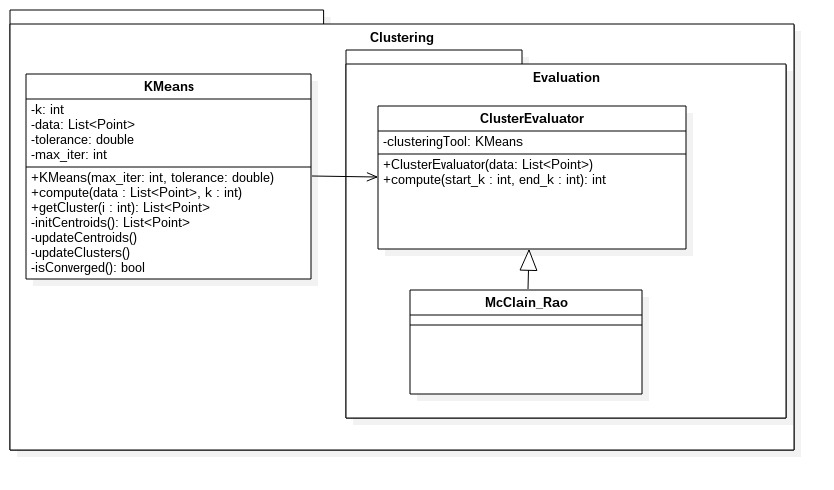
\includegraphics[width=1.0\textwidth]{../uml/classes/clustering.jpg}
    \caption{Class diagrams of clustering module}
    \label{fig:clustering_class}
\end{figure}


%---------------------------------------------------------------
%---------------------------------------------------------------

\section{Classification}

%
% CLASSIFICATION CLASS DIAGRAM
%
\begin{figure}[H]
    \centering
    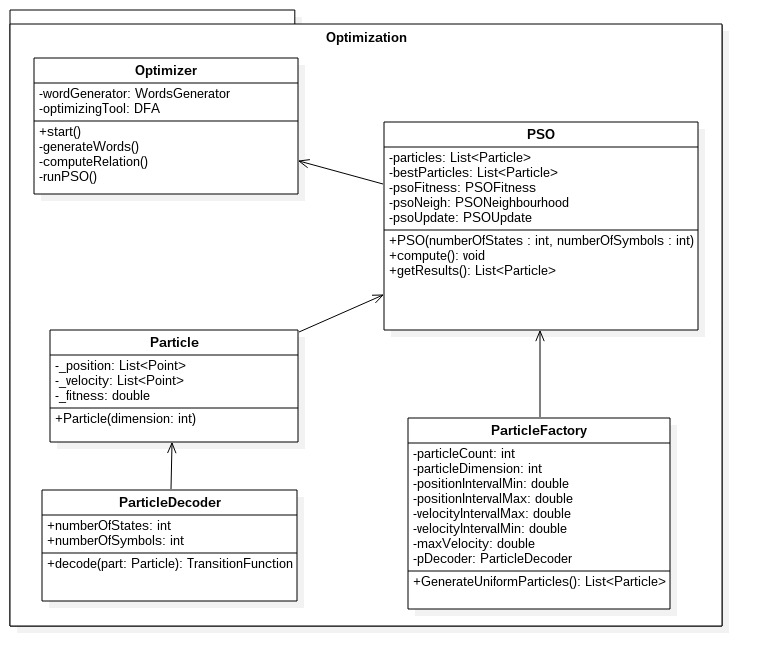
\includegraphics[width=1.0\textwidth]{../uml/classes/optimizationMain.jpg}
    \caption{Class diagrams of classification module}
    \label{fig:classification_main_class}
\end{figure}

\begin{figure}[H]
    \centering
    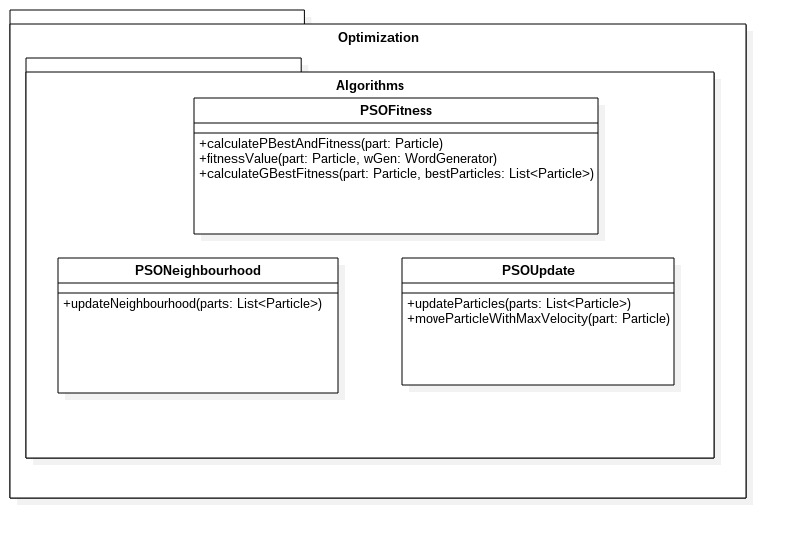
\includegraphics[width=1.0\textwidth]{../uml/classes/optimizationAlg.jpg}
    \caption{Class diagrams of classification module}
    \label{fig:classification_alg_class}
\end{figure}


%---------------------------------------------------------------
%---------------------------------------------------------------
\section{Utility}

The utility module is presented in figure~\ref{fig:utility_class}. \textit{Logger} class is responsible for printing and saving logs of the computations. It contains path to log directory and a path to specific file in which the logs should be saved. The one parameter method \textit{log}, prints the message to default file. The two parameter \textit{log} is used when the message should be saved in a different file.

The \textit{Console} class is responsible for loading flag parameters from the console, and updating the global settings. The global settings, containing all parameters of the computations are stored in \textit{Settings} class.

Finally a simple clock mechanism is proposed in \textit{Clock} class. The \textit{startClock} method starts measuring time until \textit{stopClock} is called which returns the time taken between both methods' calls. The time is encapsulated in \textit{TimeStamp} class.


%
% UTILITY CLASS DIAGRAM
%
\begin{figure}[H]
    \centering
    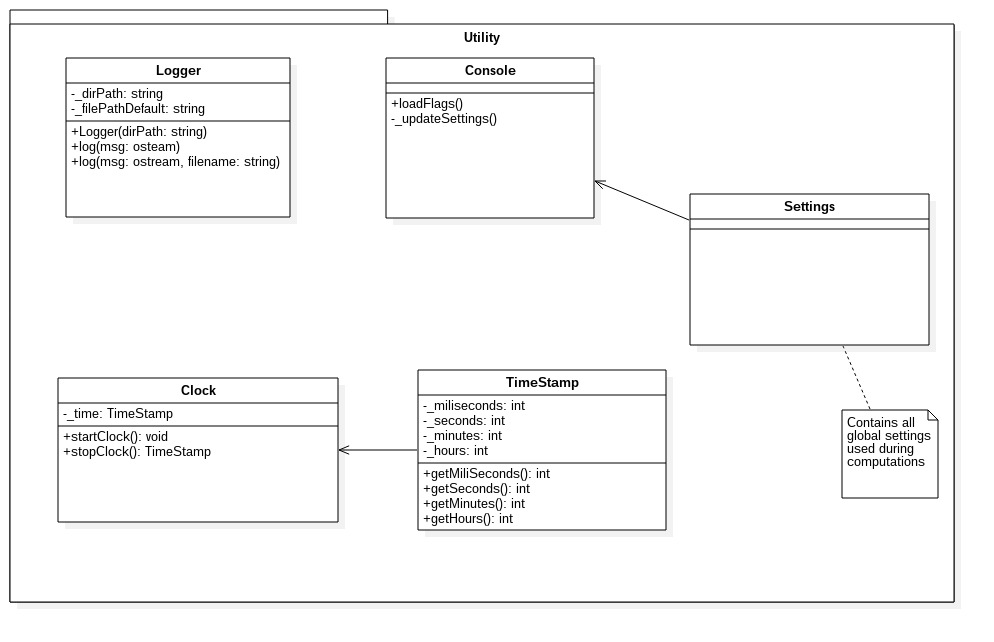
\includegraphics[width=1.0\textwidth]{images/utility_class.jpg}
    \caption{Class diagrams of utility module}
    \label{fig:utility_class}
\end{figure}







%---------------------------------------------------------------
%---------------------------------------------------------------
\section{Graphical User Interface}

%
% GUI CLASS DIAGRAM
%
\begin{wrapfigure}{c}{0.7\textwidth}
    \begin{center}
        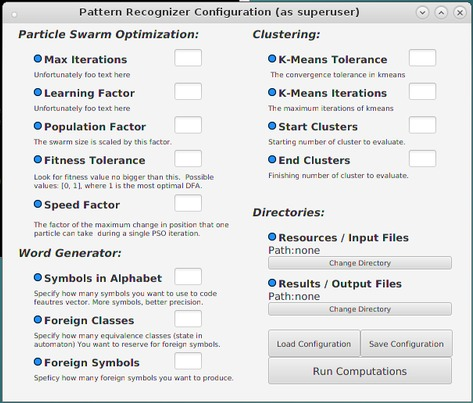
\includegraphics[width=0.7\textwidth]{images/mock_gui.jpg}
    \end{center}
    \caption{GUI Mockup}
    \label{fig:gui_look}
\end{wrapfigure}

Classes necessary to model and develop GUI are presented on figure \ref{fig:gui_classes}. On the other hand, look that we are trying to achieve is roughly sketch on figure \ref{fig:gui_look}.

As one could image, because of simplicity of the interface, there is nothing fancy in class diagram. \texttt{MainWindow} handles loading .fxml file and starting the application. On the oder hand, class \texttt{MainWindowControls} is in charge of events processing. It handles any event occurred regarding user interface objects and performs appropriate actions. Since main functionality of this part of the application is to set up global configurations, when some value within an user interface object will change, so will corresponding entry in configuration file. One can easily load and save configurations files, as well as changing directory of input and output files. Presented figure \ref{fig:gui_look}, depicting design of the application, is definitely not the final one and in future it might contain e.g. text labels with more informations about features or some loading bars. Main look of the program should be defined in .fxml, which will not be presented in this paper due to its irrelevancy and numerous way of implementations. 

\begin{figure}[H]
    \centering
    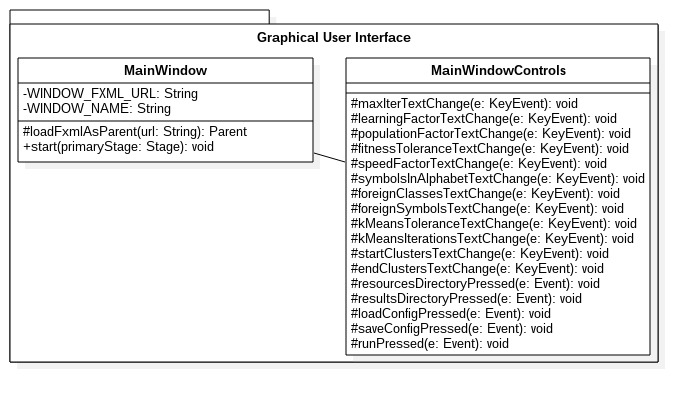
\includegraphics[width=0.9\textwidth]{images/gui.jpg}
    \caption{Class diagram of gui classes}
    \label{fig:gui_classes}
\end{figure}





%---------------------------------------------------------------
\begin{thebibliography}{1}
    
    \bibitem{pso_origin} 
    Eberhart, R. C. and Kennedy, J. A new optimizer using particle swarm theory. Proceedings of the sixth international symposium on micro machine and human science pp. 39-43. IEEE service center, Piscataway, NJ, Nagoya, Japan, 1995.
    
    %\bibitem{pso_anal}
    %Maurice Clerc. Stagnation analysis in particle swarm optimization or what happens when nothing happens, http://hal.archives-ouvertes.fr/hal-00122031. Technical report, 2006.
    
    
    
    \bibitem{pso_bias} 
    William M. Spears, Derek T. Green and Diana F. Spears. Biases in particle swarm optimization. International Journal of Swarm Intelligence Research, 1(2):34-57, 2010.
    
    
    
    
    \bibitem{pso_11}
    M. Clerc. (2011). Standard Particle Swarm Optimisation Available: http://hal.archives-ouvertes.fr/hal-00764996 
    
    \bibitem{bishop_book} Christopher M. Bishop; Pattern Recognition and Machine Learning (Information Science and Statistics)
    
	\bibitem{Homenda_2014} Homenda W., Luckner M., Pedrycz W., Classification with rejection based on various SVM techniques, Proceedings of the WCCI 2014 IEEE World Congress on Computational Intelligence, pp. 3480-3487, Beijing, China, 2014     
    
	\bibitem{semi_supervised} Xiaojin Zhu and Andrew B.Goldberg, Synthesis Lectures on Artificial Intelligence and Machine Learning, 2009, Vol. 3, No. 1 , Pages 1-130    
	
    \bibitem{semi_supervised2} Xiaojin Zhu, Semi-Supervised Learning Literature Survey, 2006

	
	\bibitem{images_learning_types} Anuj R. Shah1, Christopher S. Oehmen, Bobbie-Jo Webb-Robertson, SVM-Hustle - An iterative semi-supervised machine learning approach for pairwise protein remote homology detection 
	\bibitem{duch_uuu} Robert P.W. Duin, Elzbieta Pekalska, The Science of Pattern Recognition. Achievements and Perspectives, Studies in Computational Intelligence, chapter Challenges for Computational Intelligence, page 63 , 2007
	
\end{thebibliography}
\makestatement
\end{document}
